\documentclass[paper=a4, fontsize=11pt]{scrartcl} %twocolumn, 

\usepackage[utf8]{inputenc} % Use 8-bit encoding that has 256 glyphs

%\usepackage{fourier} % Use the Adobe Utopia font for the document - comment this line to return to the LaTeX default
\usepackage[english]{babel} % English language/hyphenation
\usepackage{amsmath,amsfonts,amsthm, amssymb} % Math packages, use \sim to get tilde

\usepackage{graphicx} % Required for including pictures

\usepackage{booktabs} % Allows the use of \toprule, \midrule and \bottomrule in tables for horizontal lines

%----------Pasting Code---------------

\usepackage{listings} % \usepackage{listings} For inserting code into the document
% Using \usepackage{listingsutf8} for multi-byte encoding of source code

\lstset{breaklines = true, 
numbers = left, 
commentstyle = \color{mygreen}, 
keywordstyle = \color{blue}, 
stringstyle = \color{mymauve},
showstringspaces = true,
basicstyle=\footnotesize
}
%inputencoding = utf8, 
%extendchars = \false

%\usepackage{minted}
\usepackage{color} %for syntax highlighting

\definecolor{mygreen}{rgb}{0,0.6,0}
\definecolor{mygray}{rgb}{0.5,0.5,0.5}
\definecolor{mymauve}{rgb}{0.58,0,0.82}

%------------END--------------

\usepackage{float} %for aligning figures

\usepackage{wrapfig} %for using wraptable or wrapfig

\usepackage{caption}
\usepackage[l2tabu]{nag}

%\usepackage[nottoc]{tocbibind} %to include the bibliography in the contents

\usepackage{verbatim} %use \begin{comment} and \end{comment}. For more complex tasks, check out package:comment

\usepackage{bm} % for printing greek symbols in bold, use \boldsymbol\varepsilon

\usepackage{rotating} % for rotating tables
\usepackage{longtable} % for long tables, 

\usepackage{subcaption} %for supressing table numbering in subtables
\usepackage{makecell} %for multiple lines in a table, enclose the cell value in \thead{A \\ B}

\usepackage{lscape} %for rotating the page with the long table

\usepackage{todonotes} %add TODOs by putting the text in \todo{}

\usepackage{csquotes} %use \begin{displayquotes} to enter a quote

% for changing the nature of urls
%\usepackage[hidelinks]{hyperref} %hides hyperlinks
\usepackage[linktoc = none, linkbordercolor	={0 1 0}]{hyperref}

% custom commands
\newcommand{\mytilde}{\raise.17ex\hbox{$\scriptstyle\mathtt{\sim}$}}

\usepackage{fancyhdr} % Custom headers and footers
\pagestyle{fancyplain} % Makes all pages in the document conform to the custom headers and footers
%\fancyhead{} % No page header - if you want one, create it in the same way as the footers below
\fancyhead[L]{}
\fancyfoot[L]{} % Empty left footer
\fancyfoot[C]{\thepage} % Page numbering for right footer
\fancyfoot[R]{} % Empty right footer
\renewcommand{\headrulewidth}{0pt} % Remove header underlines
\renewcommand{\footrulewidth}{0pt} % Remove footer underlines
\setlength{\headheight}{13.6pt} % Customize the height of the header

\numberwithin{equation}{section} % Number equations within sections (i.e. 1.1, 1.2, 2.1, 2.2 instead of 1, 2, 3, 4)
%\numberwithin{figure}{section} % Number figures within sections (i.e. 1.1, 1.2, 2.1, 2.2 instead of 1, 2, 3, 4)
%\numberwithin{table}{section} % Number tables within sections (i.e. 1.1, 1.2, 2.1, 2.2 instead of 1, 2, 3, 4)

\setlength\parindent{5pt} % Removes all indentation from paragraphs - comment this line for an assignment with lots of text

\graphicspath{{/home/ad/Desktop/images/}} % Specifies the directory where pictures are stored

%----------------------------------------------------------------------------------------
%	Some Tips For Using This Template
%----------------------------------------------------------------------------------------


\begin{comment}

\end{comment}

%----------------------------------------------------------------------------------------
%	TITLE SECTION
%----------------------------------------------------------------------------------------

\rhead{Akshat Dwivedi}
\lhead{Data Mining \& Neural Networks}
%\rfoot{\begin{picture}(0,0) \put(-45,-100){\includegraphics[width=3cm]{KU_LeuvenFR}} \end{picture}}
\newcommand{\horrule}[1]{\rule{\linewidth}{#1}} % Create horizontal rule command with 1 argument of height

\title{	
\normalfont \normalsize 
\textsc{\Large KU Leuven} \\ [30pt] % Your university, school and/or department name(s)
\horrule{0.5pt} \\[0.4cm] % Thin top horizontal rule
\huge Data Mining and Neural Networks \\ % The assignment title
\horrule{2pt} \\[0.5cm] % Thick bottom horizontal rule
}

\author{Akshat Dwivedi (Student Number: blah blah)\\
\\
Instructor: Prof. Johann Suykens\\
Course: G9X29A} % Your name

\date{January 11, 2015} % Today's date or a custom date

\pagenumbering{arabic}

%--------------------------------------------------------------------------------

\begin{document}

\maketitle % Print the title

\tableofcontents

%\thispagestyle{empty}
\clearpage
\setcounter{page}{1}

%\listoftodos %makes a list at the top of the document with TODOs

% Begin writing here:

\section{Session 1}

\subsection{Function approximation (noiseless case)}
This section involves playing with the neural network demo nndd11gn that comes with the MATLAB neural network toolbox. There are two options: selecting the number of hidden units in the network and the difficulty of the function to be approximated (scale 1-9). Index 1 corresponds to what appears to be a single sigmoid curve. The network trained on the data consists of log-sigmoid as the activation function on the units in the hidden layer. The output layer consists of one node and has the linear (identity) function as the activation function. This means that the output layer outputs without transforming the input it receives from the hidden layer. The first case (figure \ref{demo1}) compares the use of 1, 5 and 9 neurons to approximate a simple sigmoid function with difficulty index 1.

\begin{figure}[ht]
\centering
	\begin{subfigure}[b]{0.3\textwidth}
		\centering
		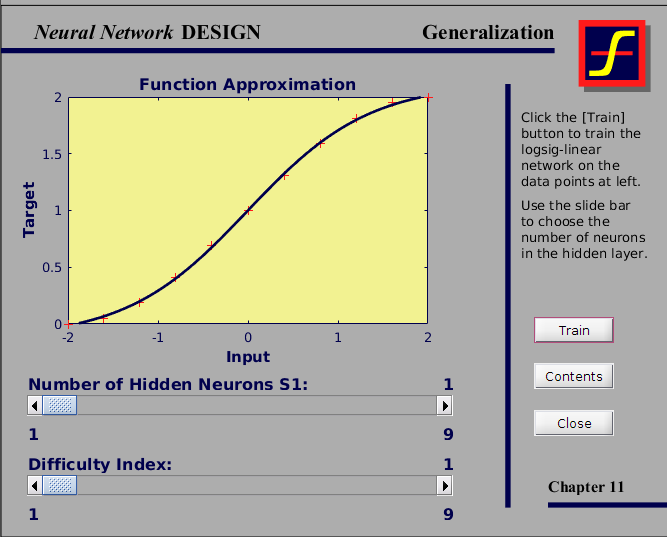
\includegraphics[width = \textwidth]{d11.png}
		\caption{Index = 1, neurons = 1}
	\end{subfigure}
	\begin{subfigure}[b]{0.3\textwidth}
		\centering
		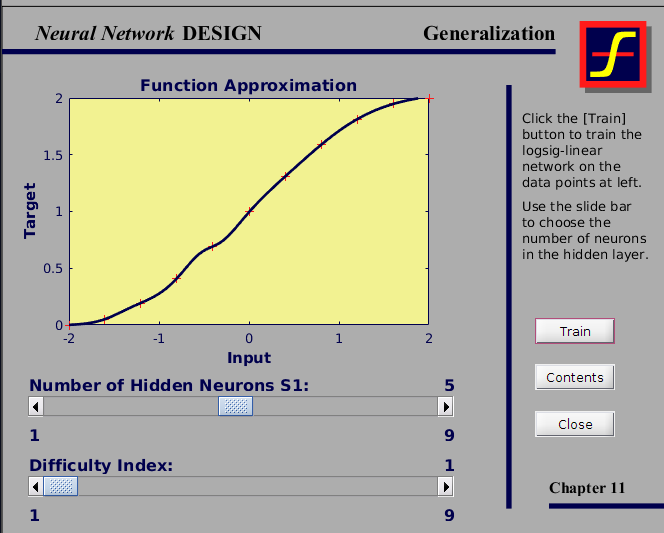
\includegraphics[width = \textwidth]{d15.png}
		\caption{Index = 1, neurons = 5}
	\end{subfigure}
	\begin{subfigure}[b]{0.3\textwidth}
		\centering
		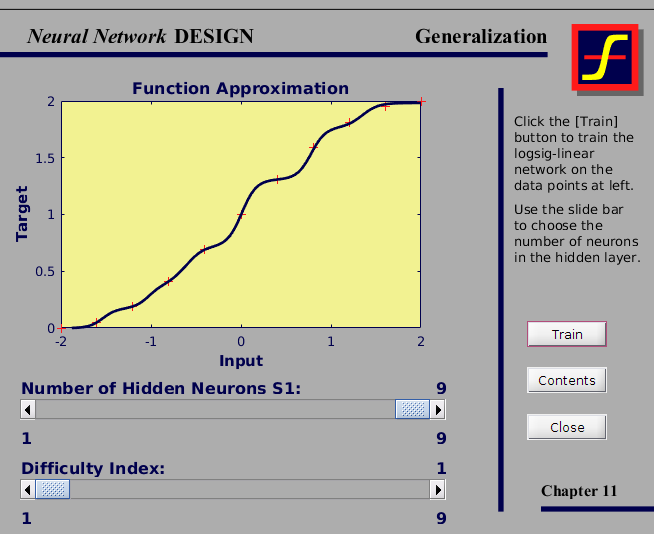
\includegraphics[width = \textwidth]{d19.png}
		\caption{Index = 1, neurons = 9}
	\end{subfigure}
\caption{Neural network demo nnd11gn}
\label{demo1}
\end{figure}

In figure \ref{demo1}, we see that 1 neuron is sufficient to approximate the original function and the curve is rather smooth. In case of 5 or 9 neurons, the approximated curve is overfitting the data which is indicated by the bumps in the approximated function. 

\begin{figure}[ht]
\centering
	\begin{subfigure}[b]{0.3\linewidth}
		\centering
		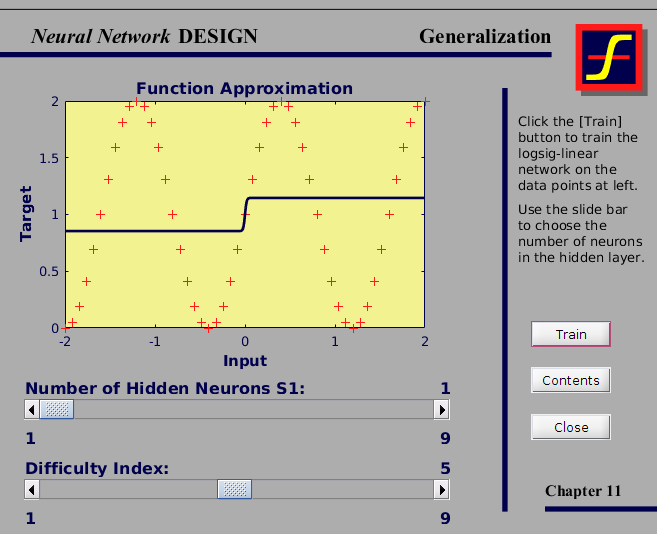
\includegraphics[width = \textwidth]{d51.png}
		\caption{Index = 5, neurons = 1}
	\end{subfigure}
	\begin{subfigure}[b]{0.3\linewidth}
		\centering
		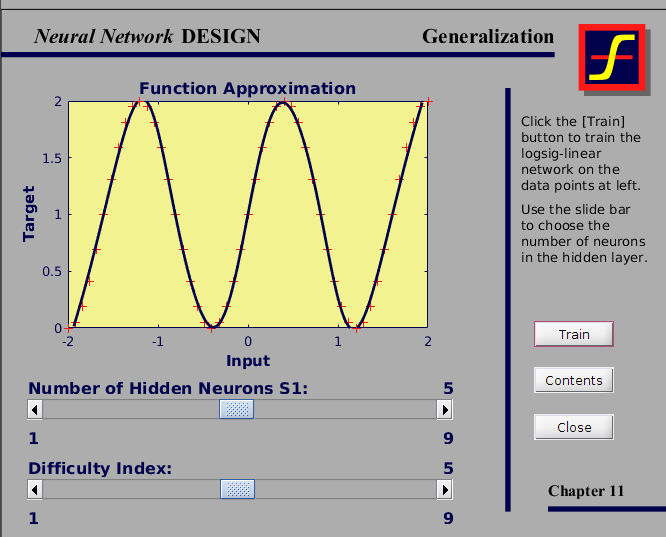
\includegraphics[width = \textwidth]{d55.png}
		\caption{Index = 5, neurons = 5}
	\end{subfigure}
	\begin{subfigure}[b]{0.3\linewidth}
		\centering
		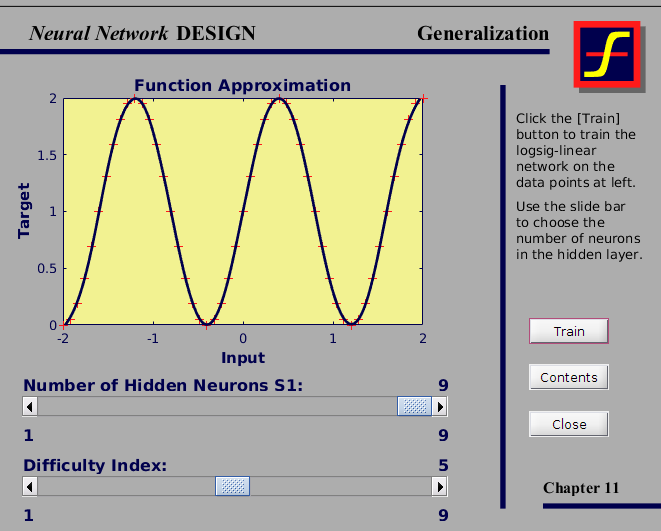
\includegraphics[width = \textwidth]{d59.png}
		\caption{Index = 5, neurons = 9}
	\end{subfigure}
\caption{Neural network demo nnd11gn}
\label{demo2}
\end{figure}

In figure \ref{demo2}, we see that using 1 neuron is insufficient to approximate the underlying function (after multiple epochs). Using 5 neurons is sufficient to approximate the underlying function (although there were a few cases where the optimization algorithm reached a local minima and the network failed to approximate the function.) This is a well-known drawback of using neural networks. The network was able to capture the underlying relationship in the data with 9 neurons across multiple epochs. This would usually lead to overfitting, unless regularization was used to keep the network weights small or some form of pruning were applied after training the network.

\begin{figure}[ht]
\centering
	\begin{subfigure}[b]{0.3\linewidth}
		\centering
		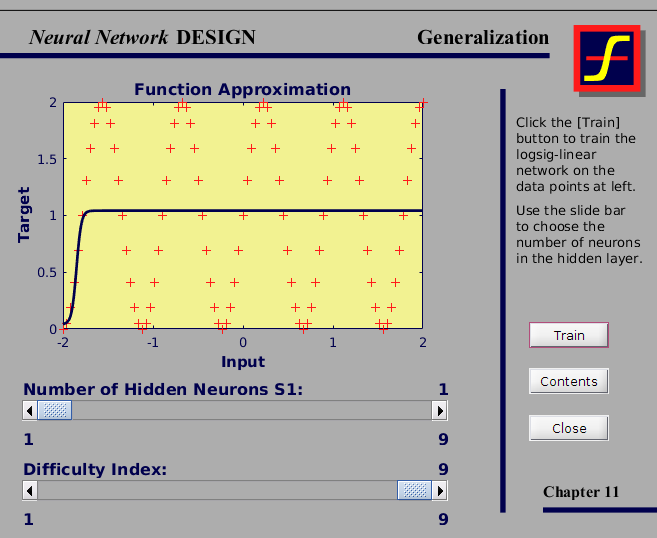
\includegraphics[width = \textwidth]{d91.png}
		\caption{Index = 9, neurons = 1}
	\end{subfigure}
	\begin{subfigure}[b]{0.3\linewidth}
		\centering
		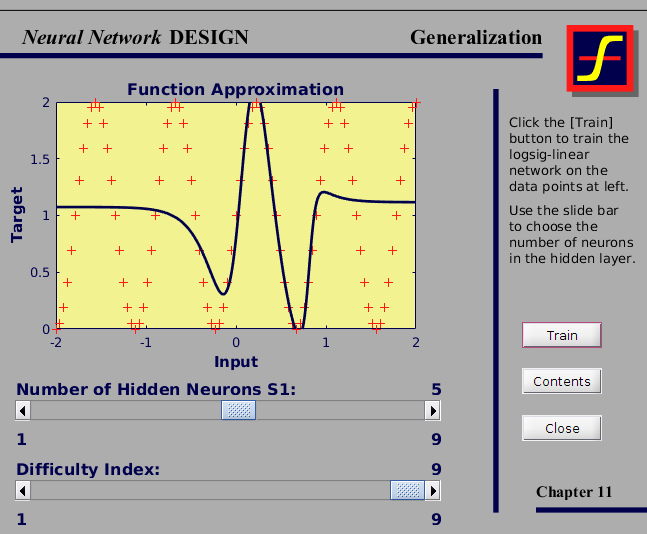
\includegraphics[width = \textwidth]{d95.png}
		\caption{Index = 9, neurons = 5}
	\end{subfigure}
	\begin{subfigure}[b]{0.3\linewidth}
		\centering
		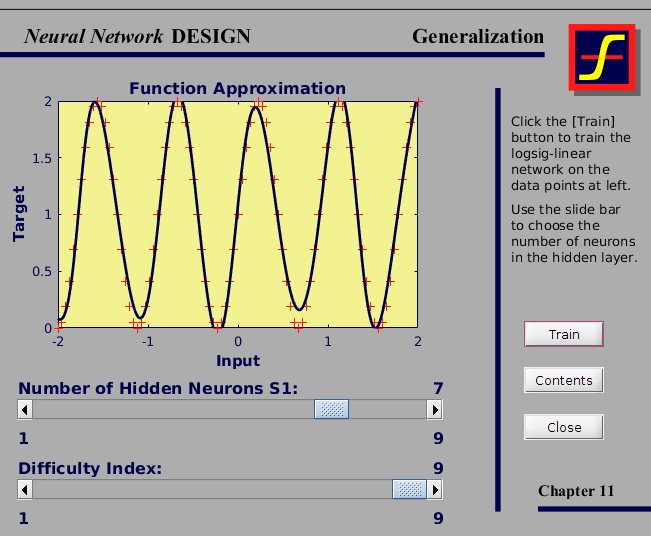
\includegraphics[width = \textwidth]{d97.png}
		\caption{Index = 9, neurons = 7}
	\end{subfigure}
\caption{Neural network demo nnd11gn}
\label{demo3}
\end{figure}

Finally, we consider the case with the maximum difficulty index: 9. Based on figure \ref{demo3}, we see that 1 neuron is completely insufficient for approximating the true function. 5 neurons is insufficient to approximate the function as well, however, it is able to approximate a part of the true function. We do not show the 9 neuron case, but instead, show that 7 neurons was sufficient to approximate the underlying function in about 80\% of the cases. Adding 8 or 9 neurons would only improve this number. Lastly, one should be careful at deriving rules of thumbs based on this demo, as the underlying function did not have any noise in the data, and the number of observations available in the training set would affect the training and the architecture of the network as well.\\

The under/over fitting is due to the number of hidden units and the activation function employed. In the 5 or 9 index case, the underlying function appears sinusoidal. Thus, using a sinusoid as an activation function can reduce the number of hidden units required to approximate the true function, compared to the sigmoid function that was used. However, the sinusoidal function is not monotonic, and hence the universal approximation theorem does not guarantee that one can learn the function by using this activation function (monotonicity of the activation function is a requirement of the theorem).

\subsection{The role of the hidden and output layers}

Linear (ordinary least-squares) regression can be performed by using the simplest neural network architecture, which is composed of a single hidden layer comprising a single node with a linear activation function and training using squared error loss. The input layer has $p$ nodes (the number of features or columns in the dataset) and the network has one output neuron in the output layer. Sometimes, an additional bias term can be added to the input layer as well, in which case the input layer has $p+1$ nodes. The input to the network is a collection of $n$ p-dimensional vectors. Thus, $n$ is the number of records or observations, and $p$ is the columns of the data matrix. Symbolically, it can be written as

\begin{align}
y \quad = \quad \sigma(w^Tx+\beta)
\end{align}

where $\sigma(w^Tx+\beta) = w^Tx+\beta$ is the linear (identity) activation function, 

\begin{align}
w^Tx + \beta \quad = \quad w_1x_1 + \ldots + w_px_p + \beta
\end{align}

and $\beta$ is the bias (threshold) term. 

\begin{figure}[ht]
\centering
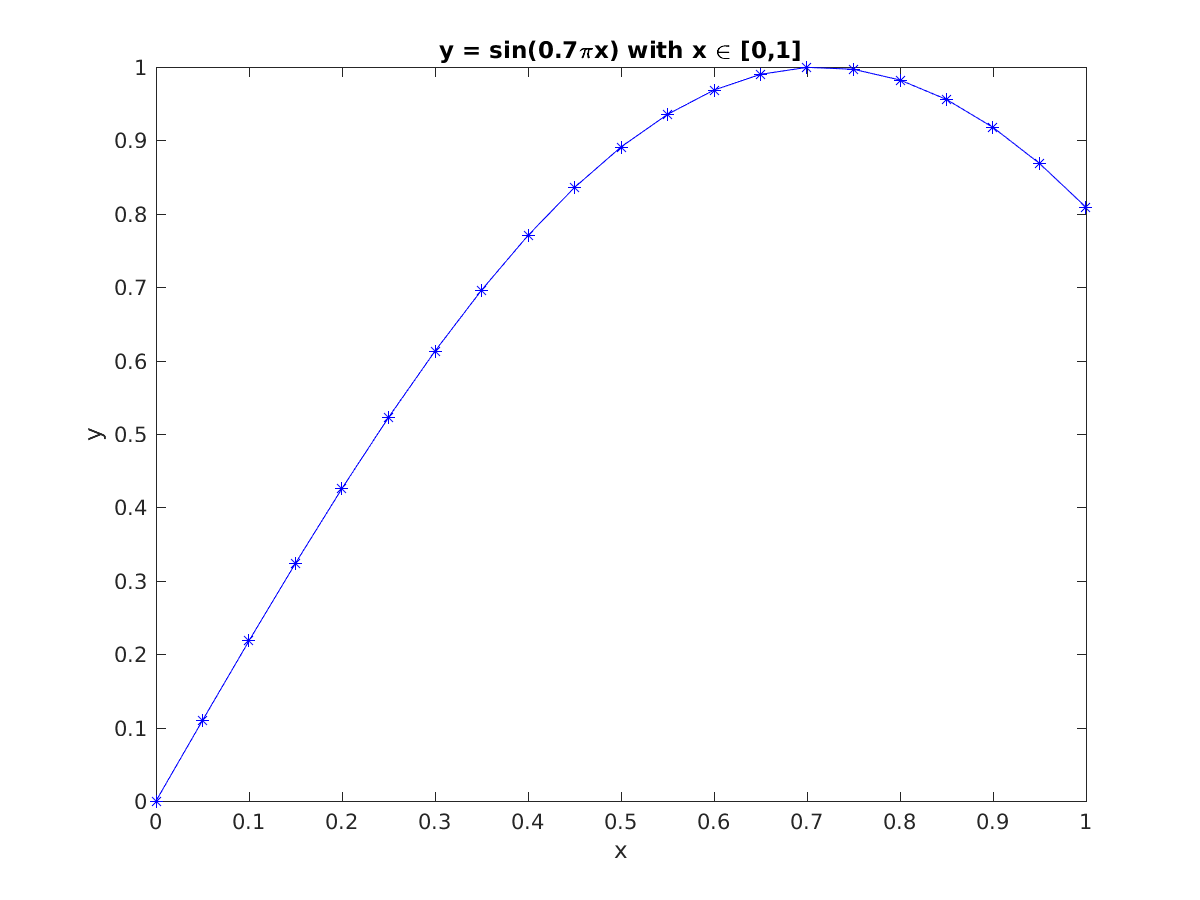
\includegraphics[scale = 0.35]{sinpix.png}
\caption{Plot of y = sin(0.7$\pi$x) vs x}
\label{sinpix}
\end{figure}

Figure \ref{sinpix} contains a plot of the function $y_p = \textrm{sin}(0.7 \pi x_p)$ where $x_p \in [0,1]$, i.e., 21 equally spaced points between 0 and 1. Since this function is nonlinear, linear regression as described in the starting paragraph will not be able to capture the true underlying relation between the inputs and the outputs.\\

We first train a network with two neurons in the hidden layer using the above values of $x$ and $y.$ The biases for the two hidden neurons $b_1$ = -1.7735 and $b_2$ = 0.0982; and the weights $w_1$ = 1.3714 and $w_2$ = -1.2680. The inputs to the network were not scaled before training. The activation function on the neurons in the hidden layer is the hyperbolic tangent function [2/1+exp(-2n)]-1. The activation function for the output layer is the linear/identity function which mirrors the information from the hidden layer to the single node in the output layer.\\

\begin{figure}[ht]
\centering
	\begin{subfigure}[b]{0.3\textwidth}
	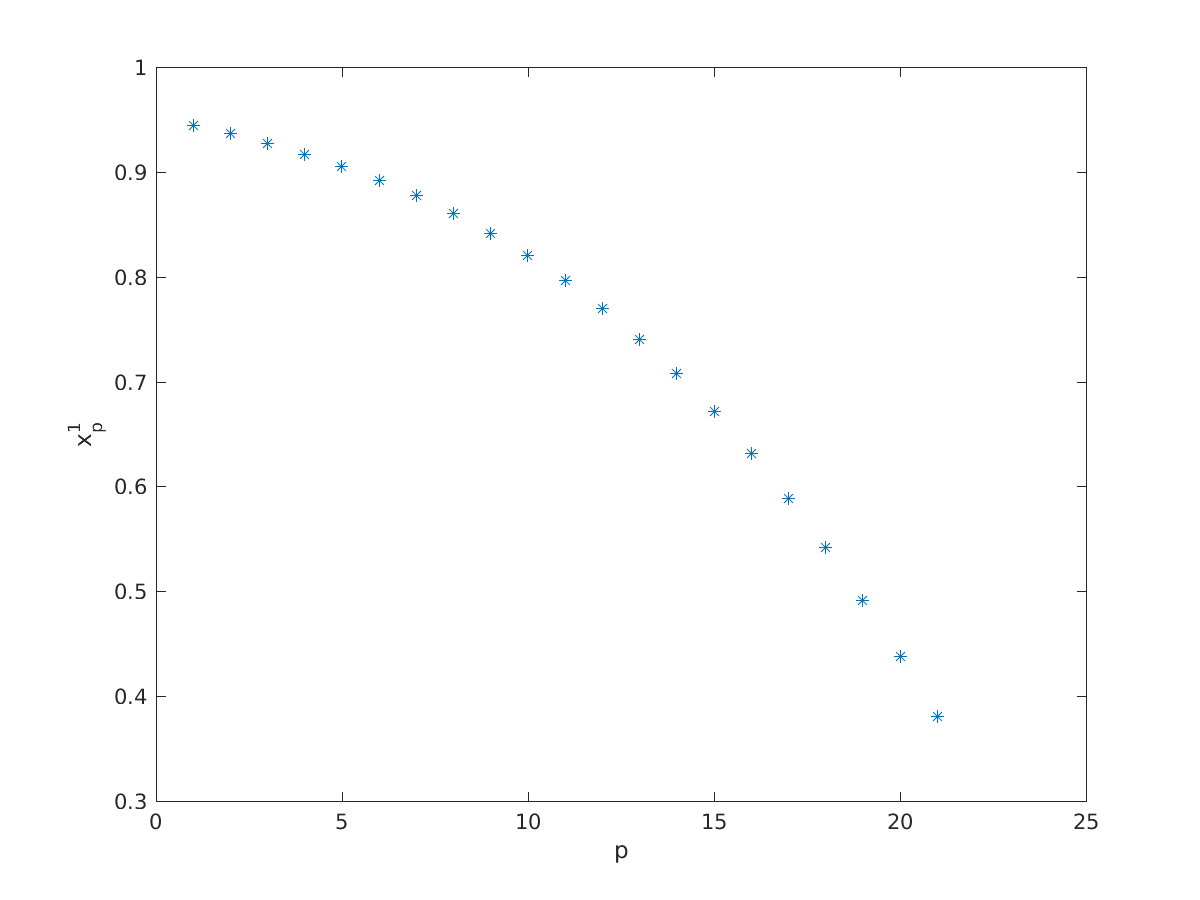
\includegraphics[width = \textwidth]{x1p.png}
	\caption{x$_p^1$}
	\end{subfigure}
	\begin{subfigure}[b]{0.3\textwidth}
	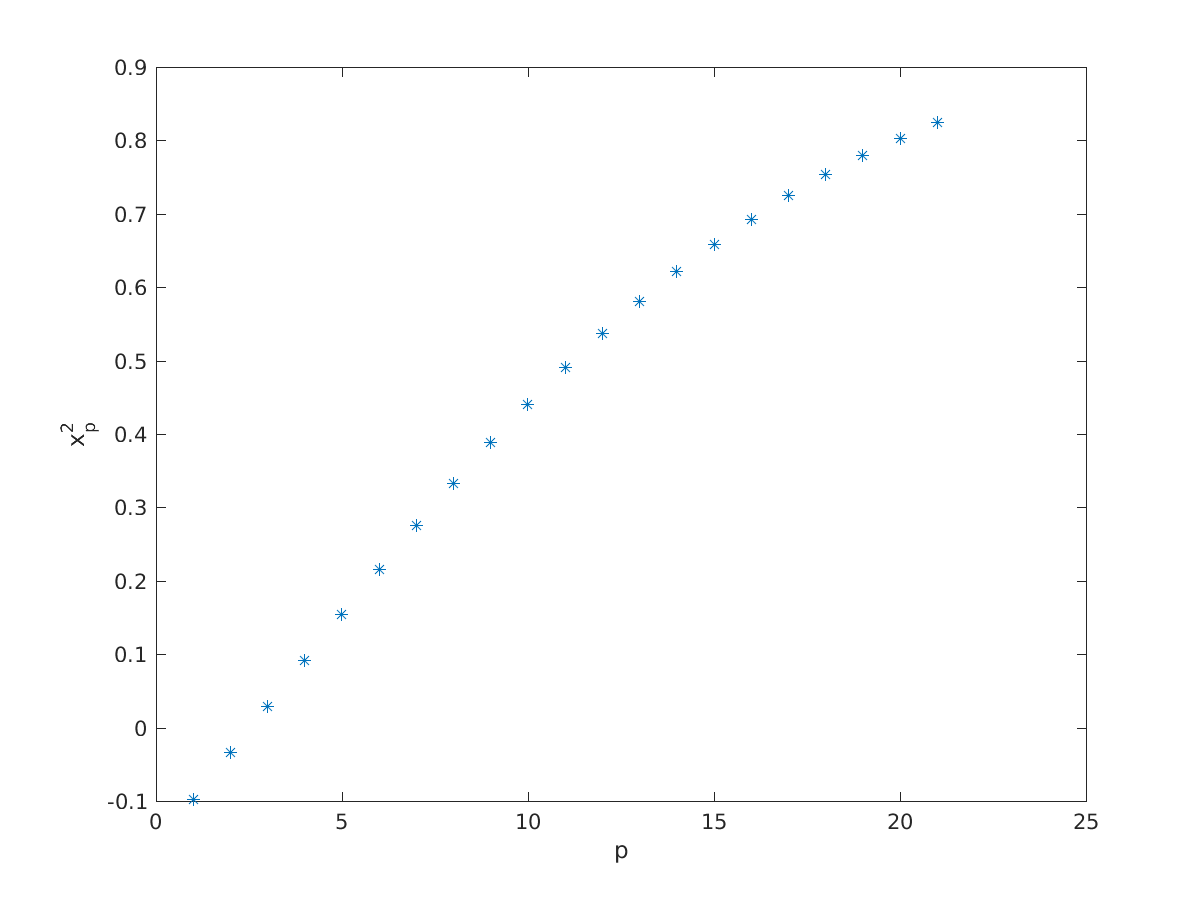
\includegraphics[width = \textwidth]{x2p.png}
	\caption{x$_p^2$}
	\end{subfigure}
		\begin{subfigure}[b]{0.3\textwidth}
	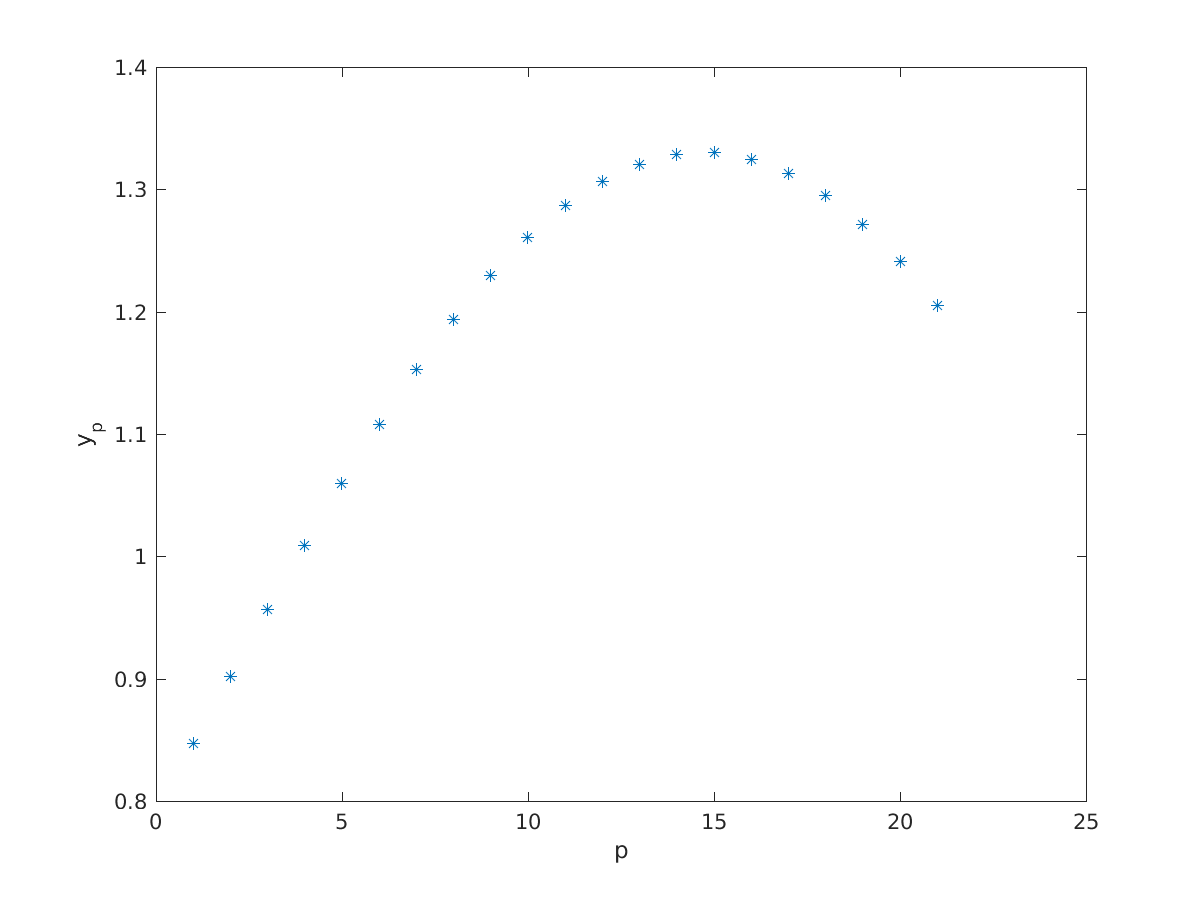
\includegraphics[width = \textwidth]{yp.png}
	\caption{$y_p = x_p^1 + x_p^2$}
	\end{subfigure}
\caption{Plot of $x_p^1$ $x_p^2$ and $y_p$ against $p = 1, \ldots,21$}
\label{xp}
\end{figure}

Figure \ref{xp} shows a plot of $x_p^1$, $x_p^2$ and $y_p$ against $p = 1, \ldots,21$. Here we see parts of the true function that are approximated by the two neurons $x^1$ and $x^2$. Individually, either neuron cannot model the true function, however part (c) shows that a linear combination of the two neurons (with unit weights) does capture the true relationship. Notice that the $y$-axis shows the function outside the range of the original $y$. This is because we have not yet taken a weighted combination of the neurons yet. The final output from the network is plotted in figure \ref{output}.

\begin{figure}[ht]
\centering
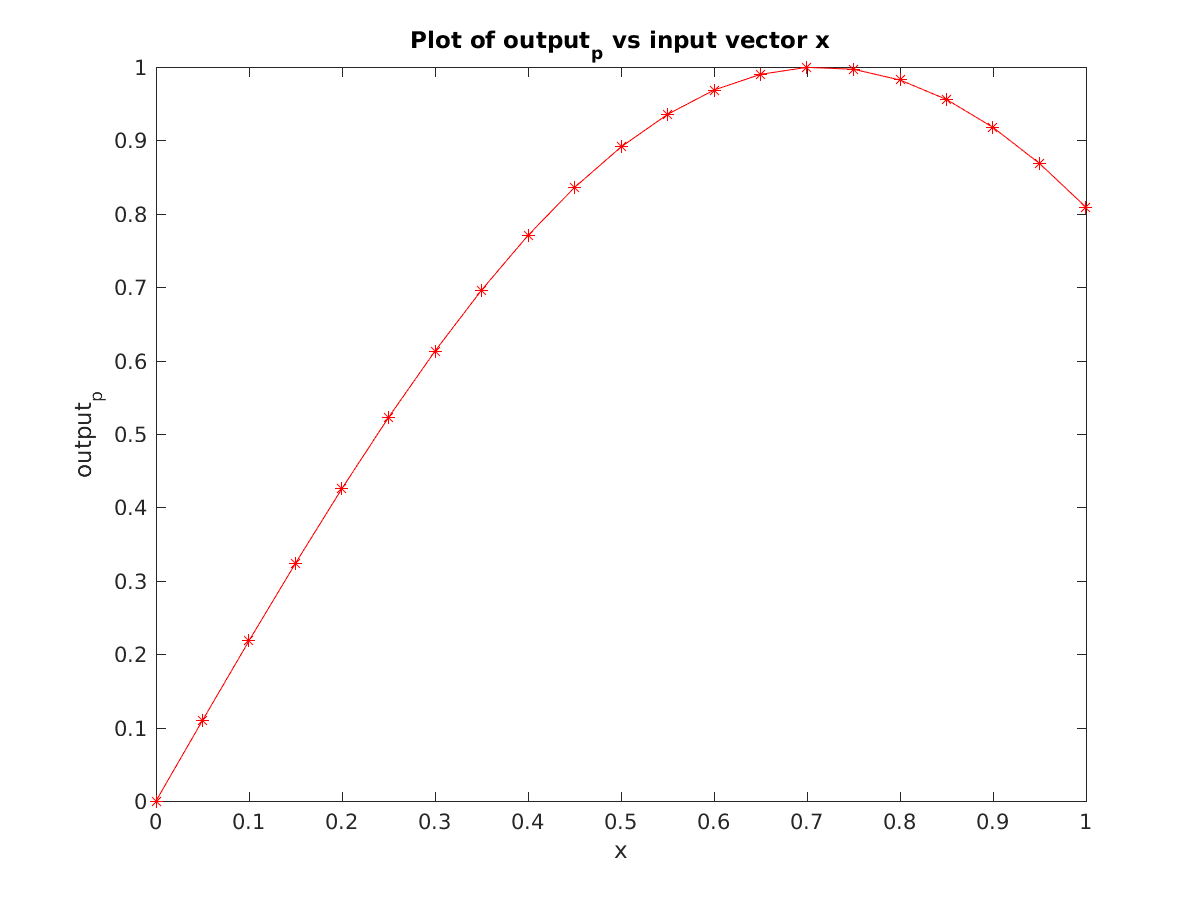
\includegraphics[width = 0.5\textwidth]{outputp.png}
\caption{Plot of output$_p$ vs. x$_p$. This is indistinguishable from the original target $\mathtt{y}$.}
\label{output}
\end{figure}

\subsection{Function approximation (noisy case)}
For this part, a training set of a sinusoidal signal sin(2$\pi$x) on [-1,1] with additional Gaussian noise is generated with 50, 200 and 1000 observations. A validation set is chosen to be of the same size as the training set with the sinusoidal signal on [-0.9,0.9] with additional Gaussian noise as well. Three different levels of noise $\sigma$ are chosen, namely 0.1, 1.0 and 2.0 for simulating the Gaussian error $\varepsilon$ $\mytilde$ $N(0,\sigma)$. Regularization ($0.8, 0.3$ and $10^{-4}$) or early stopping were used while training the network and a multi-layer perceptron with a single hidden layer with 5, 10 and 20 neurons was used. \\

The primary training algorithm used was the Levenberg-Marquadt algorithm (LM) which was chosen due to its fast convergence. The division of the training and the validation sets were done using fixed indices, which eliminates the variability from random division of the dataset into training and validation sets before training the network. The initial seed and the random number generator were fixed at the start. This allows us to make all the comparisons without worrying about additional sources of variability as all sources of variability have been eliminated for these comparisons and the results can be reproduced using the code given in the appendix.\\

\begin{figure}[ht]
\centering
	\begin{subfigure}[b]{0.3\textwidth}
	\centering
	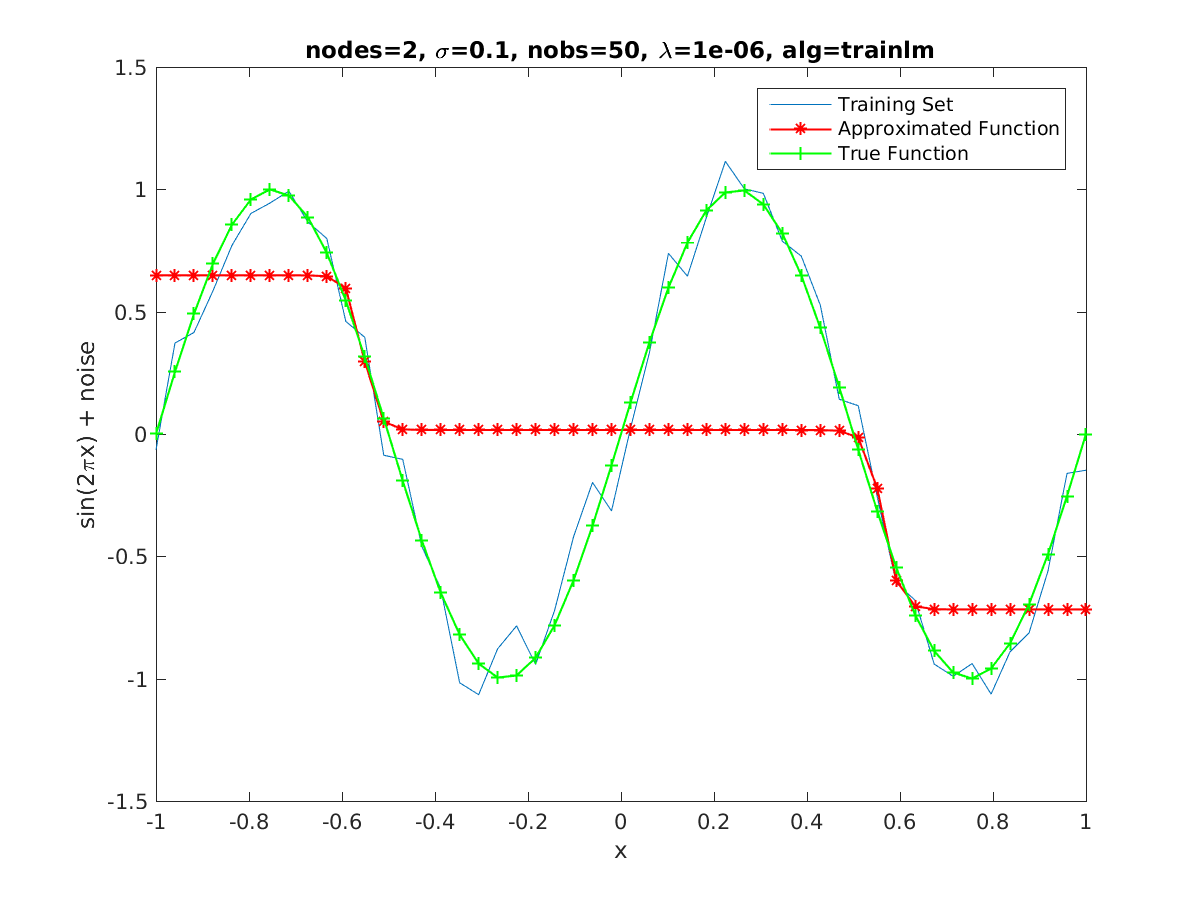
\includegraphics[width = \textwidth]{a.png}
	\caption{$n_h=2$, n = 50}
	\end{subfigure}
\begin{subfigure}[b]{0.3\textwidth}
	\centering
	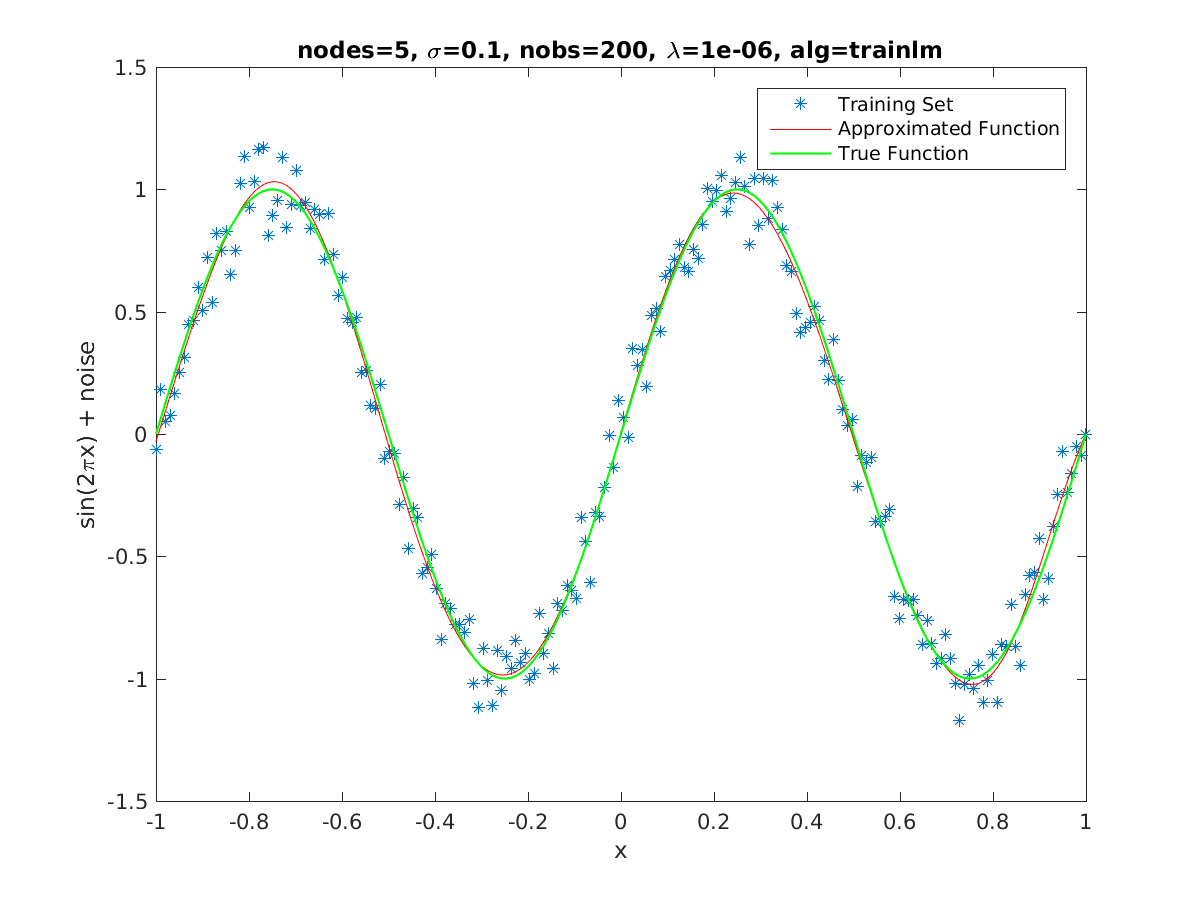
\includegraphics[width = \textwidth]{b.png}
	\caption{$n_h=5$, n = 200}
	\end{subfigure}
\begin{subfigure}[b]{0.3\textwidth}
	\centering
	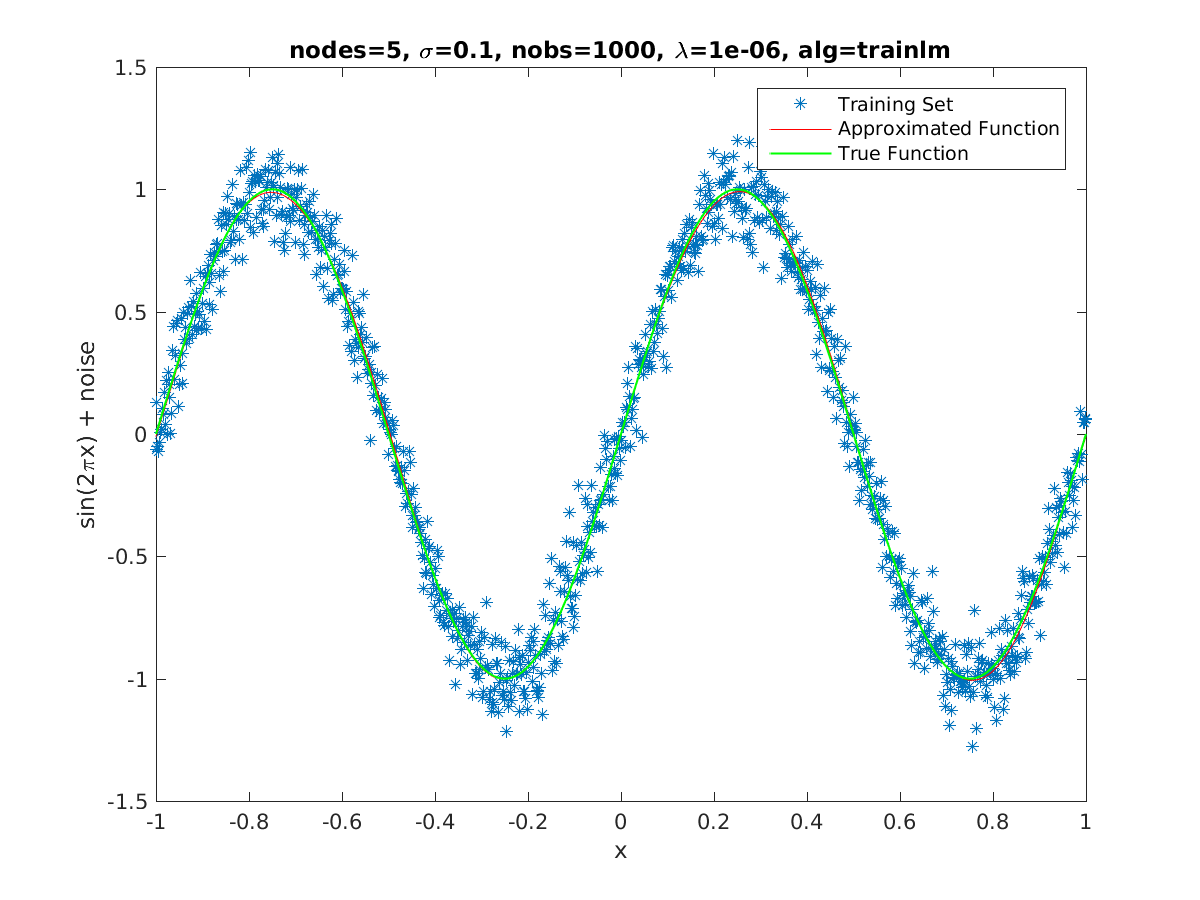
\includegraphics[width = \textwidth]{c.png}
	\caption{$n_h=5$, n = 1000}
	\end{subfigure}
\caption{LM algorithm, noise $\sigma=0.1$ and using early stopping.}
\label{nobs1}
\end{figure}

In figure \ref{nobs1}, we  compare the cases with 50, 200 and 1000 observations. The first image was fit with 2 neurons, however, this resulted in a poor fit and the number of neurons after this were taken to be 5 (except for the sections on regularization and comparing different number of hidden units). The noise is fixed at $\sigma=0.1$ and we see that the noisy function does not deviate too much from the true function. In the second part, we see that with 200 observation, the network is able to approximate the true function and this accuracy is improved with 1000 observations (part (c)). This would indicate that the presence of noise can be overcome with more data.

\begin{figure}[ht]
\centering
	\begin{subfigure}[b]{0.3\textwidth}
	\centering
	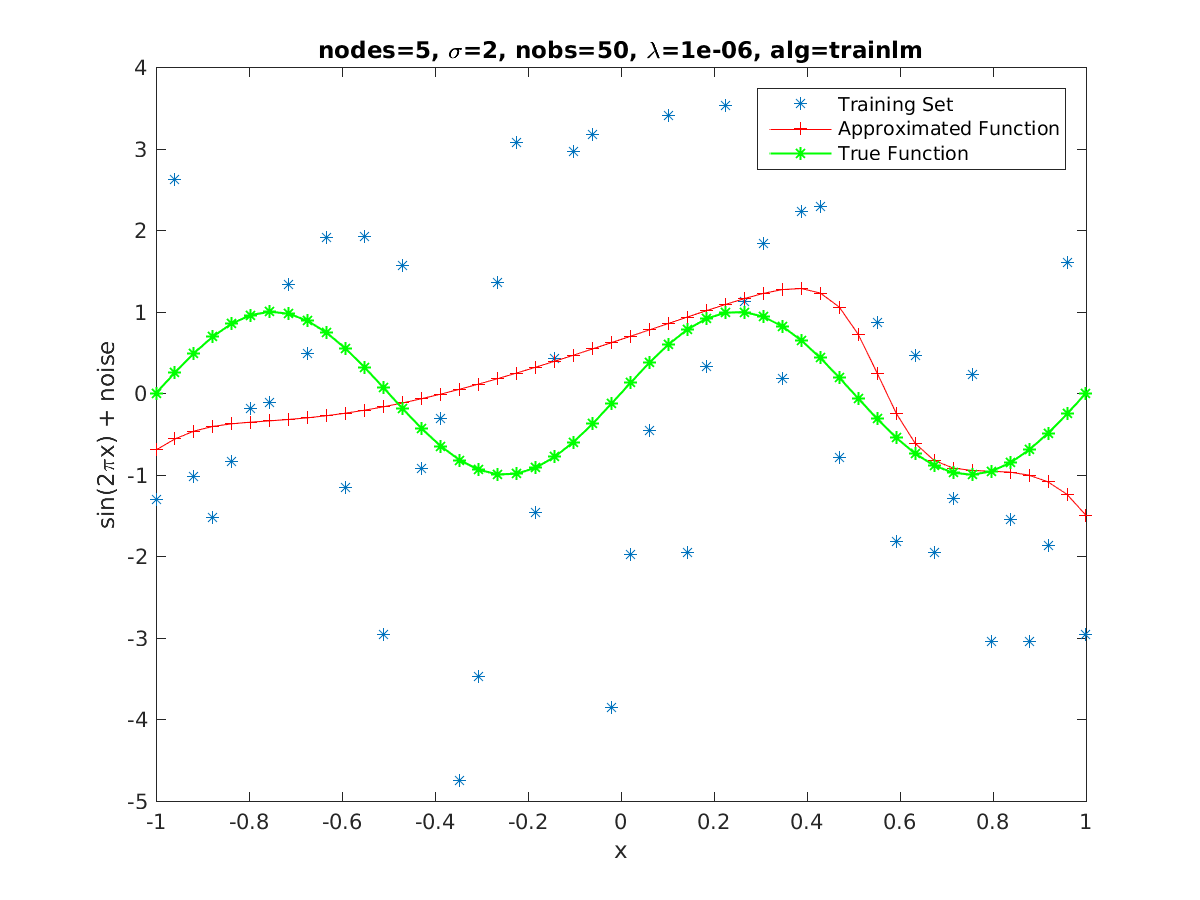
\includegraphics[width = \textwidth]{d.png}
	\caption{n = 50}
	\end{subfigure}
\begin{subfigure}[b]{0.3\textwidth}
	\centering
	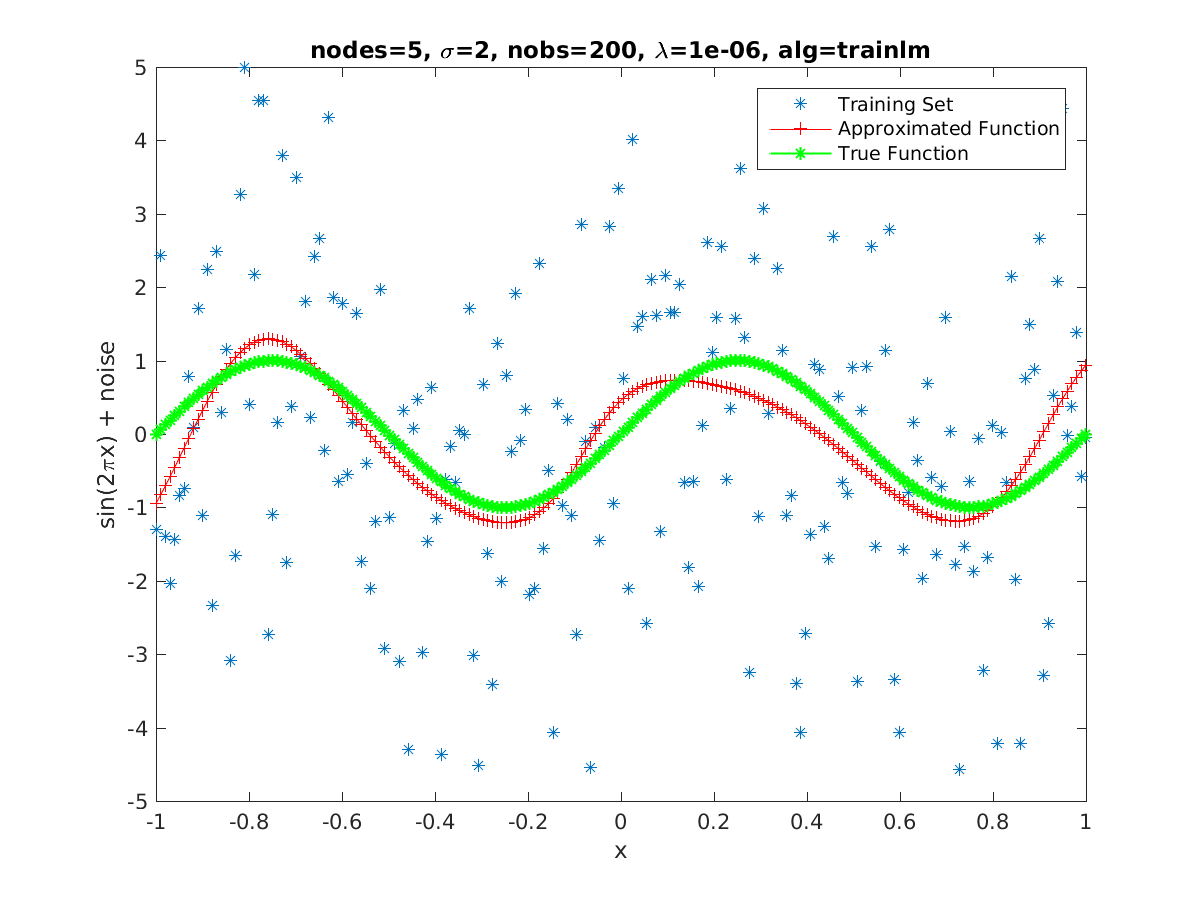
\includegraphics[width = \textwidth]{e.png}
	\caption{n = 200}
	\end{subfigure}
\begin{subfigure}[b]{0.3\textwidth}
	\centering
	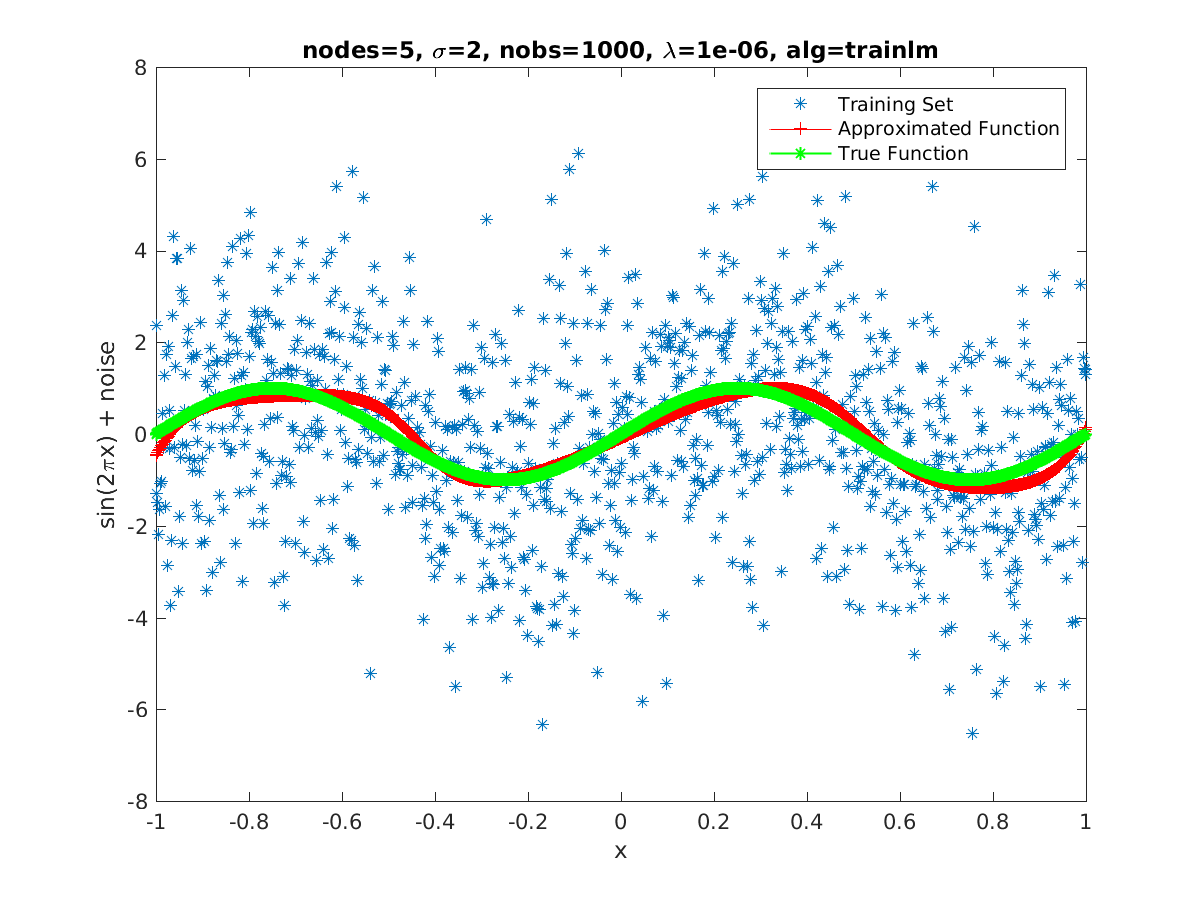
\includegraphics[width = \textwidth]{f.png}
	\caption{n = 1000}
	\end{subfigure}
\caption{noise $\sigma=2.0$, $n_h$ = 5, early stopping.}
\label{nobs2}
\end{figure}

In figure \ref{nobs2}, we see that with a large amount of noise ($\sigma=2.0$) and a small number of observations, the network is unable to approximate the underlying process with 5 neurons, as it was able to before. However, with increasing cases (200 and 1000), the network improves at approximating the underlying function.\\

\begin{figure}[ht]
\centering
	\begin{subfigure}[b]{0.3\textwidth}
	\centering
	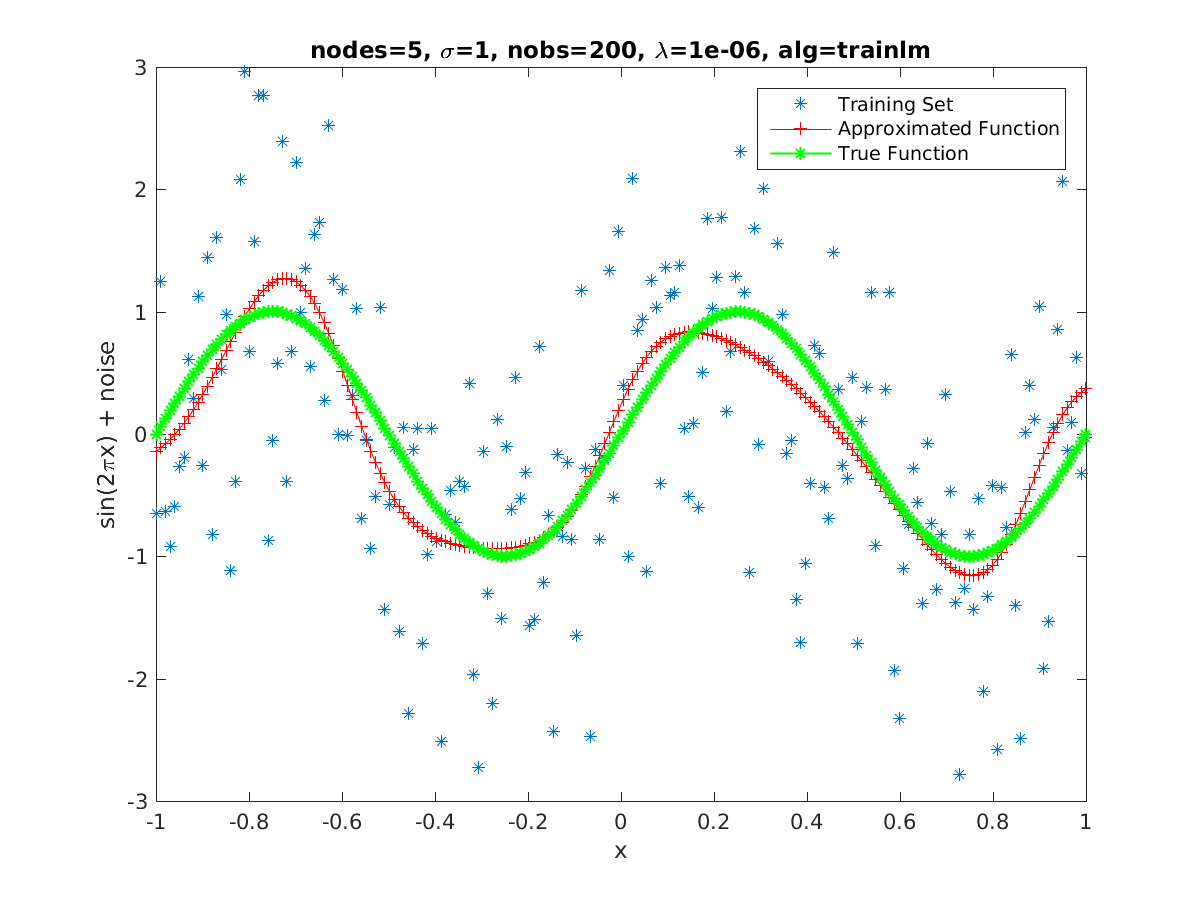
\includegraphics[width = \textwidth]{g.png}
	\caption{$n_h$ = 5}
	\end{subfigure}
\begin{subfigure}[b]{0.3\textwidth}
	\centering
	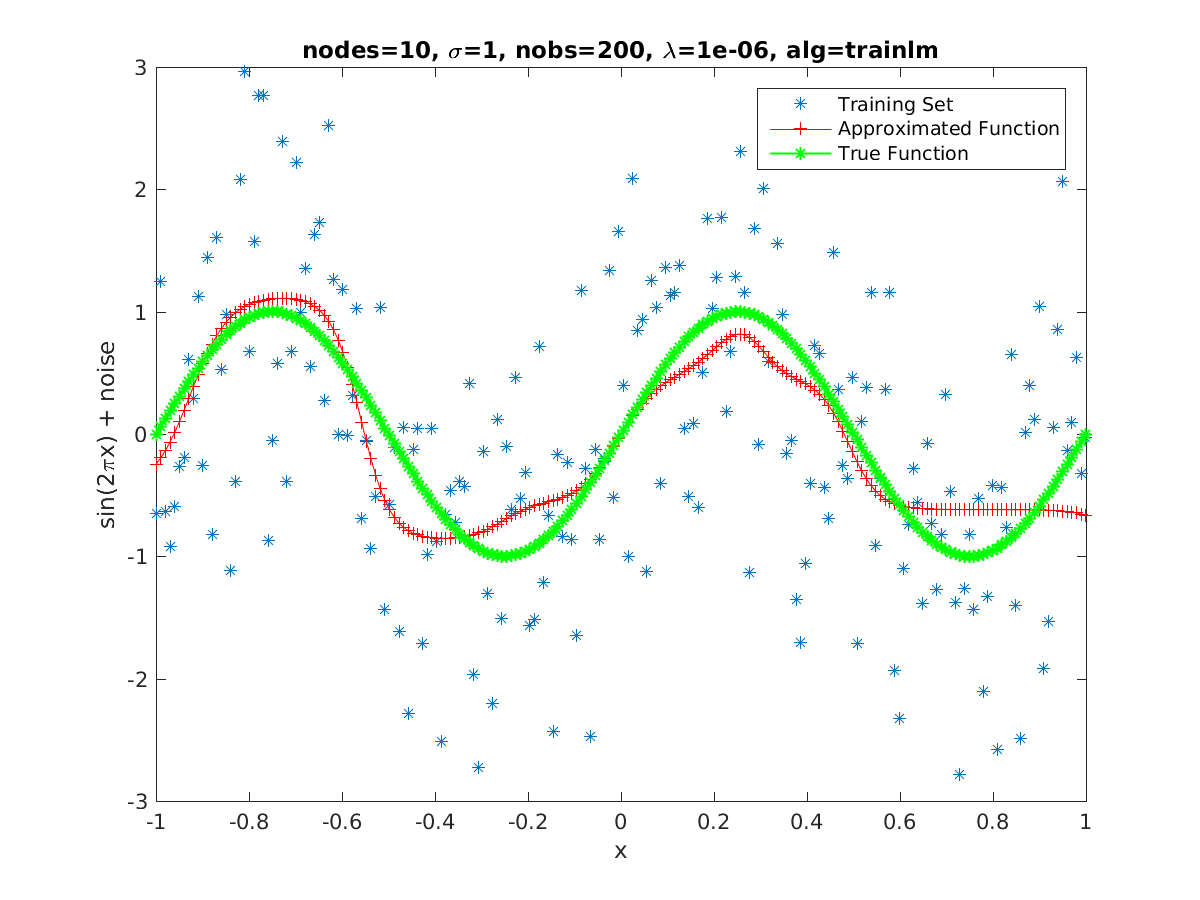
\includegraphics[width = \textwidth]{h.png}
	\caption{$n_h$ = 10}
	\end{subfigure}
\begin{subfigure}[b]{0.3\textwidth}
	\centering
	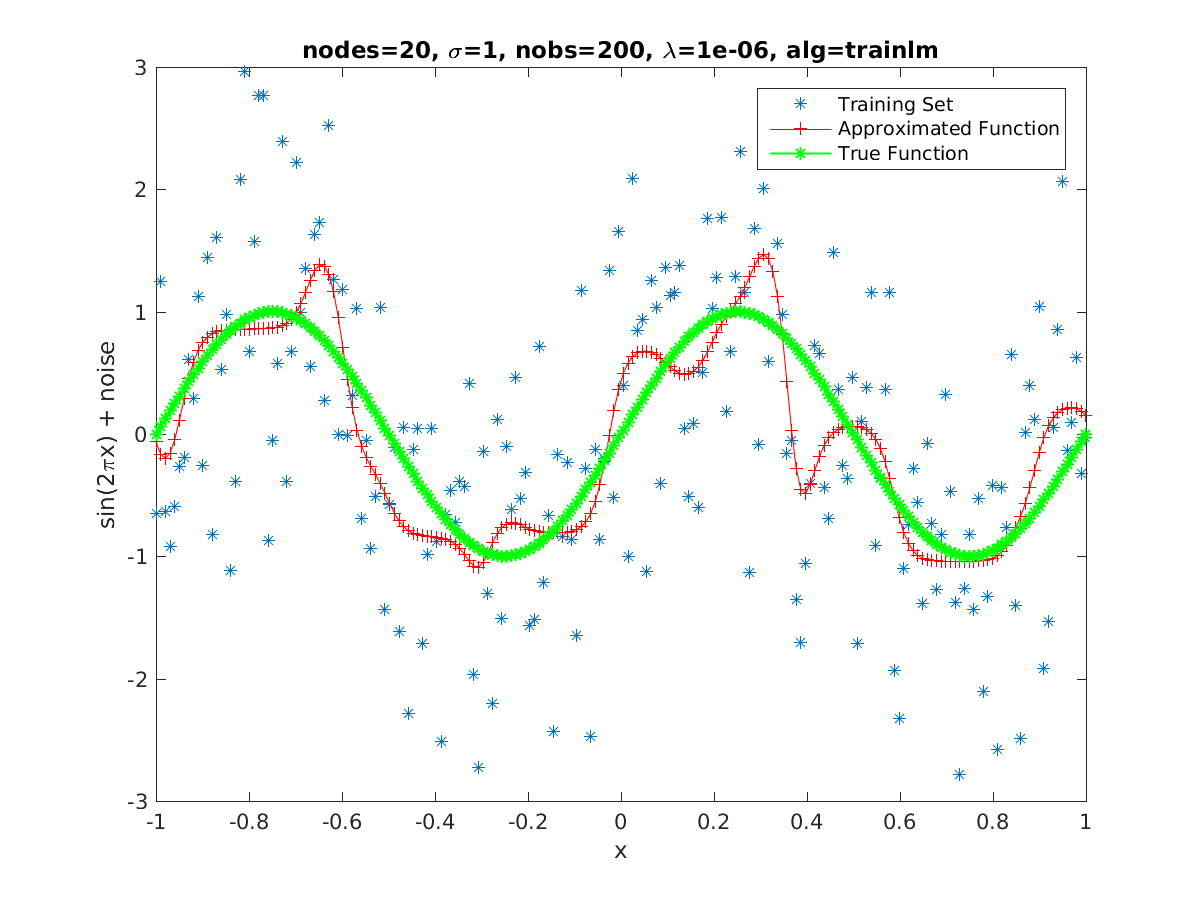
\includegraphics[width = \textwidth]{i.png}
	\caption{$n_h$ = 20}
	\end{subfigure}
\caption{Comparing the number of hidden units. Noise $\sigma=1.0$ and n = 200 are fixed.}
\label{nhidden}
\end{figure}

This third figure \ref{nhidden} compares the accuracy of the network with different hidden units. The figures with 5 and 10 neurons are still relatively close to the true function, however, we see that adding more neurons leads to the network overfitting to the given training set, although it still models the general shape of the true function.\\

\begin{figure}[ht]
\centering
	\begin{subfigure}[b]{0.3\textwidth}
	\centering
	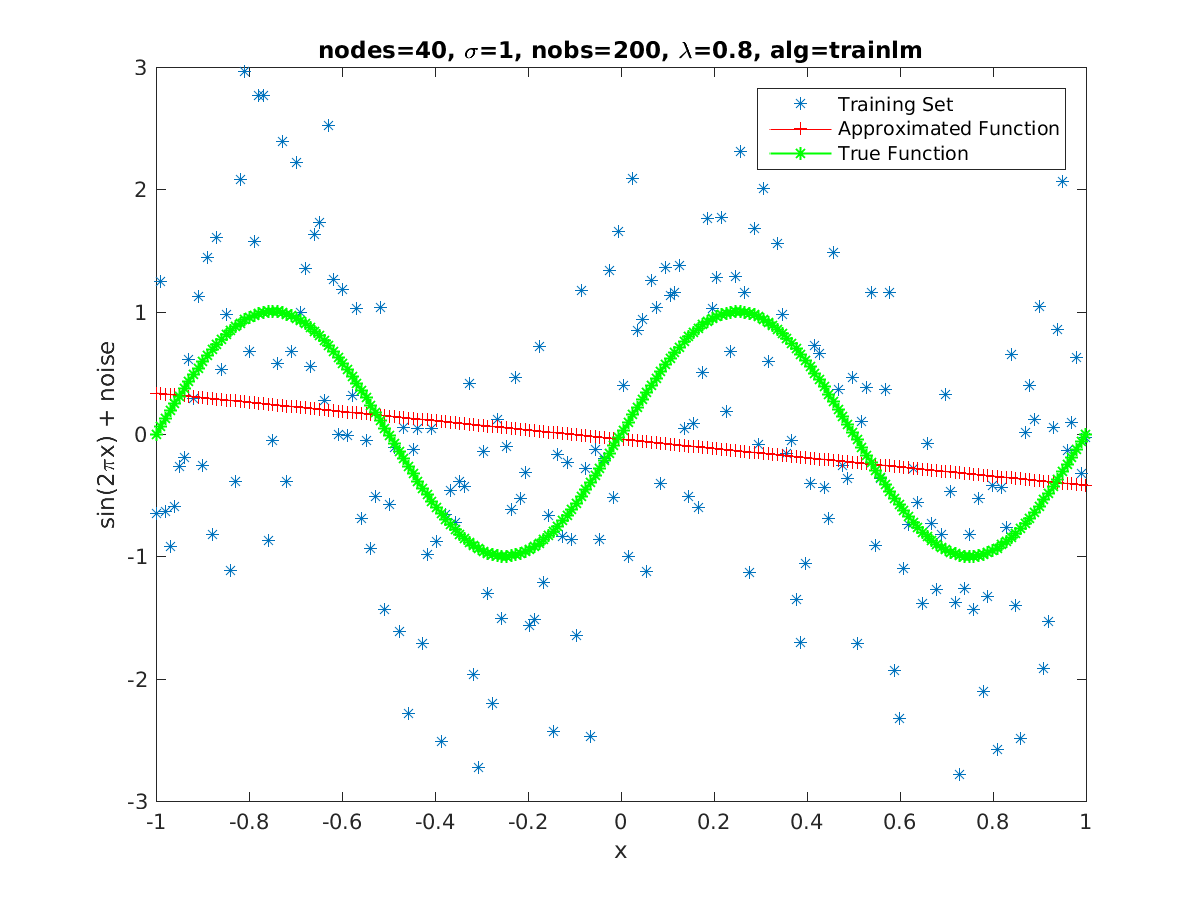
\includegraphics[width = \textwidth]{j.png}
	\caption{$\lambda = 0.8$}
	\end{subfigure}
\begin{subfigure}[b]{0.3\textwidth}
	\centering
	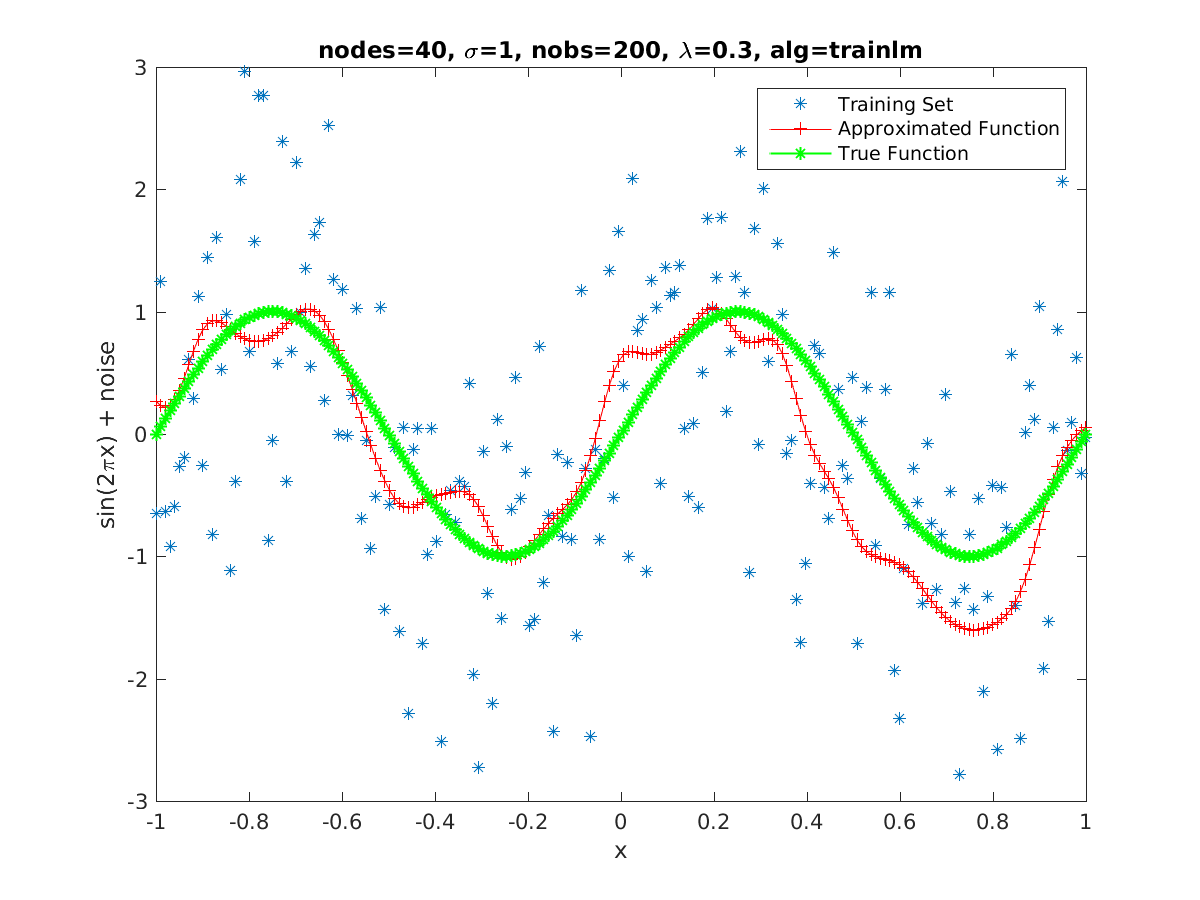
\includegraphics[width = \textwidth]{k.png}
	\caption{$\lambda = 0.3$}
	\end{subfigure}
\begin{subfigure}[b]{0.3\textwidth}
	\centering
	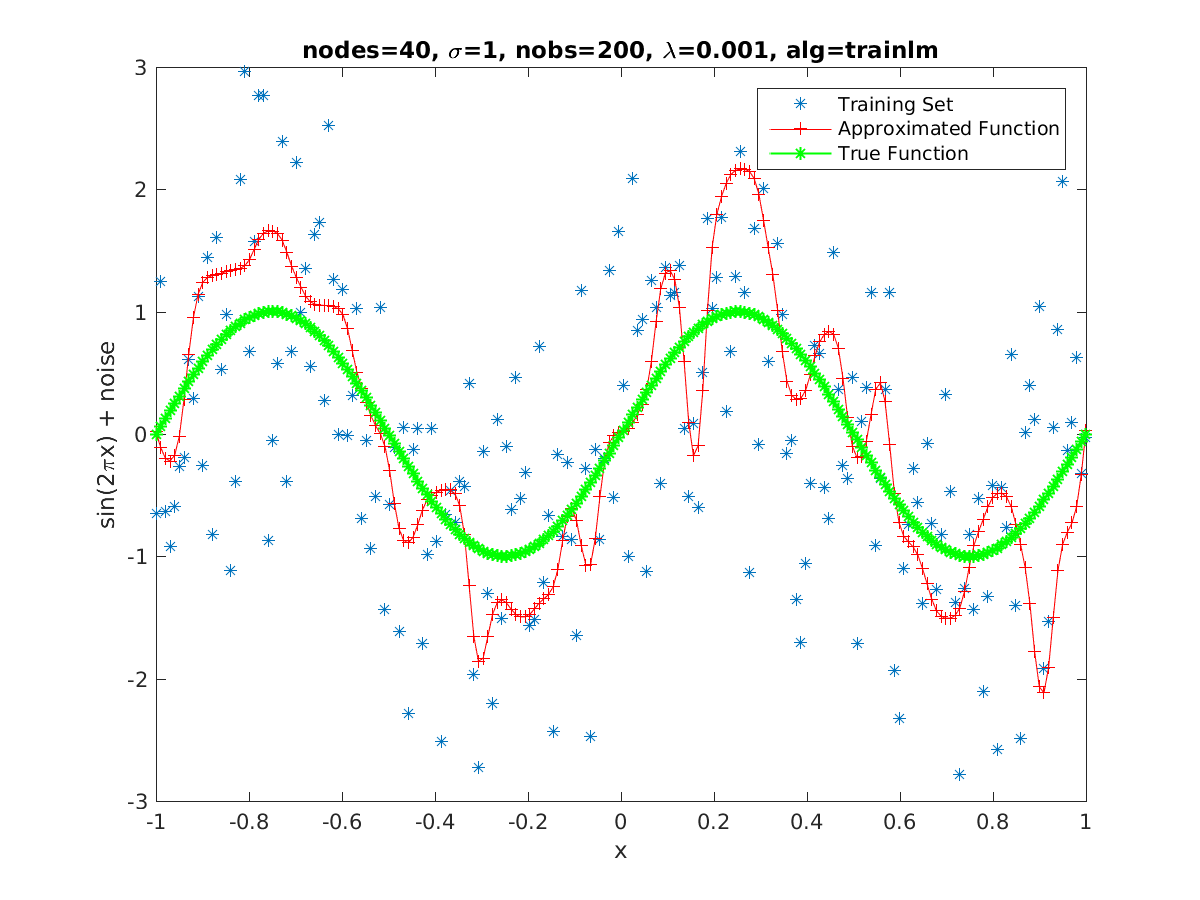
\includegraphics[width = \textwidth]{l.png}
	\caption{$\lambda = 10^{-4}$}
	\end{subfigure}
\caption{$\sigma=1.0$, $n_h = 40$, \textbf{regularization $\lambda$}, n = 200}
\label{regular}
\end{figure}

The fourth figure \ref{regular} assess the impact of choosing an appropriate regularization parameter. The figure on the left shows too much regularization ($\lambda=0.8$) which results in a large bias in the approximated function and fails to approximate the true function. The approximation function in the middle ($\lambda=0.3$) appears to give a decent approximation to the true function, however, it is still learning patterns in the data that are a result of noise (random fluctuations) and not due to the underlying process. The third figure results in too little regularization ($\lambda = 10^{-4}$) which results in a large variance in the approximated function but little bias. The approximated function is overfitting the training data and is failing to obtain a good generalization. Thus, the middle figure appears to be a decent example of the bias-variance trade-off. Selecting a $\lambda$ value between 0.3 and 0.6 should most likely result in a good fit to the data.\\

\begin{table}[ht]
\centering
\begin{tabular}{c|c|c|c|c}
\hline
Algorithms & \thead{Levenberg-\\Marquadt} & \thead{Scaled Conjugate \\Gradient} & \thead{BFGS \\ quasi-Newton} & \thead{resilient \\ backpropagation} \\
\hline
\thead{$n_h=5$ \\ epochs = 200} & 25s & 21s & 39s & 11s \\
\hline
\thead{$n_h=40$ \\ epochs = 50} & 39s & 25s & 59s & 13s \\
\hline
\end{tabular}
\caption{Comparing the training times (in seconds) of the different algorithms. Early stopping and regularization were not used; only runtimes were of interest. n = $10^6$, noise $\sigma=1.0$ and number of hidden units (5 and 40) were held fixed.}
\label{algorithm}
\end{table}

This final comparison uses the LM, SCG, BFGS and resilient backpropagation algorithms for training the network. The number of cases were increased to $10^6$ instead of 1000. Although there was only one feature, adding more features to the dataset would enable us to distinguish between the algorithms to a greater degree. The noise level was fixed at 1.0, and $n_h$ was 5 (case 1) and 40 (case 2). All the networks were trained without regularization or early stopping and for a fixed number of epochs (case 1: 200) and (case 2: 50). From table \ref{algorithm}, we see that based on runtimes, resilient backpropagation is the fastest, with scaled conjugate gradient coming in second place. Thus, for much larger datasets, it would make sense to use the resilient backpropagation alogorithm.

\subsection{Curse of dimensionality}
Our aim in this part is to model the popular $y=sinc(x)$ function for $x \in \mathbb{R}^m$, m = 1, 2 and 5 dimensions using a neural network.

\subsubsection*{Case m = 1}
First, we create a training set and a test set. The training set comprises of 100 equally spaced points on [-5,5] starting at -5. For selecting the test set from the same interval, we try to ensure that there is no overlap between the training and the test sets. For this, we can choose $n_{\mathrm{test}}$ from [-5,5] by using a number that is coprime to 100. We take 53 equally spaced points on the interval [-4.9,4.9] starting at the end point -4.9. This results in the training set A ($\subset$ [-5,5]) and test set B ($\subset$ [-4.9,4.9]) being mutually disjoint. This is shown in figure \ref{sinc1}.

\begin{figure}[ht]
\centering
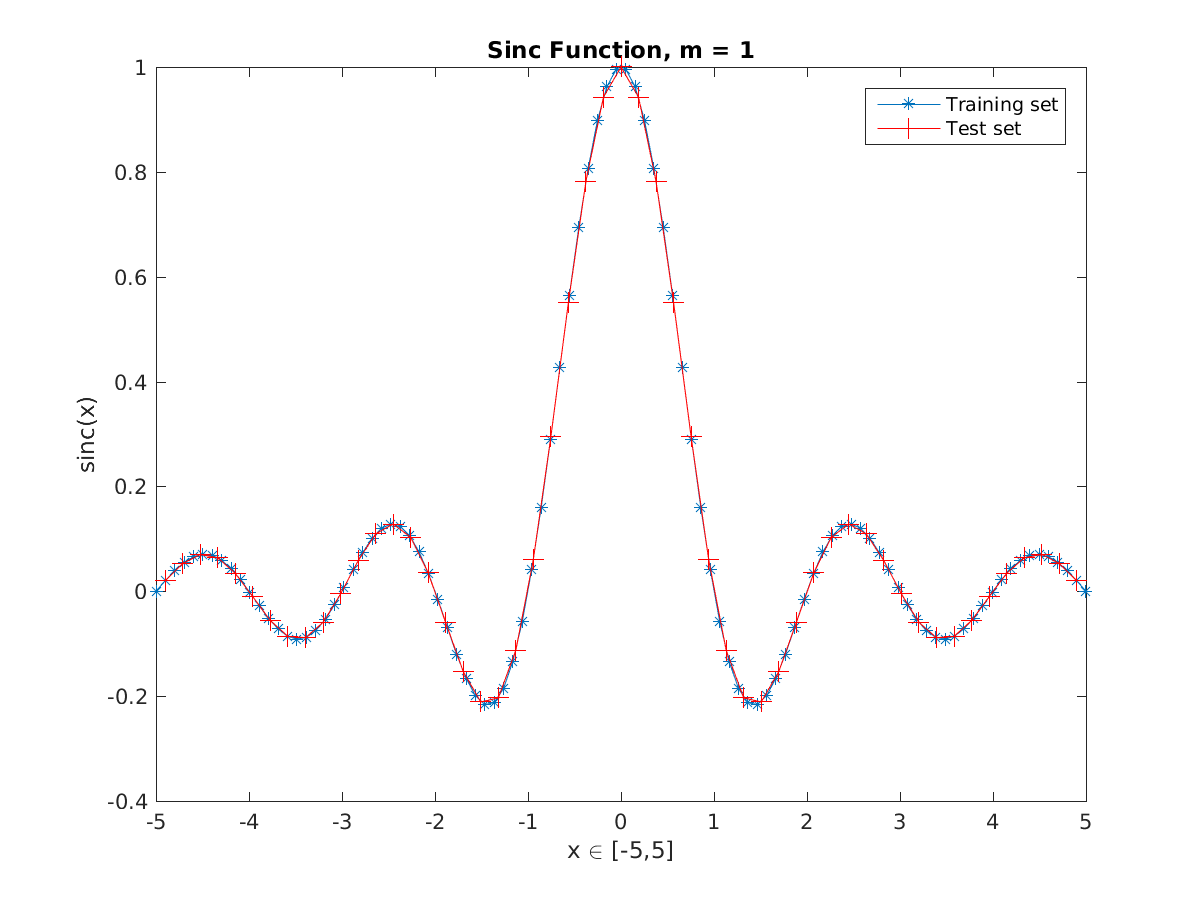
\includegraphics[width = 0.5\textwidth]{sinc1.png}
\caption{Plot of the 1-dimensional sinc(x) function for x. Training set is from [-5,5] and test set is from [-4.9,4.9]. Both sets are mutually disjoint.}
\label{sinc1}
\end{figure}

Figure \ref{sinc1} contains a plot of the training and the test sets. We train two MLPs on the training set with one hidden layer and 5 neurons. The difference between the two networks is that the first one uses the hyperbolic tan function as the activation function and the second one uses the radial basis function. Figure \ref{sinc1fit} shows the differences in the approximated functions from these two networks. The network with the tanh activation provides a poorer fit for $x>3.8$. We prefer to go with the radial basis network as it provides a better fit with a smaller number of neurons.

\begin{figure}[ht]
	\begin{subfigure}[b]{0.5\textwidth}
		\centering
		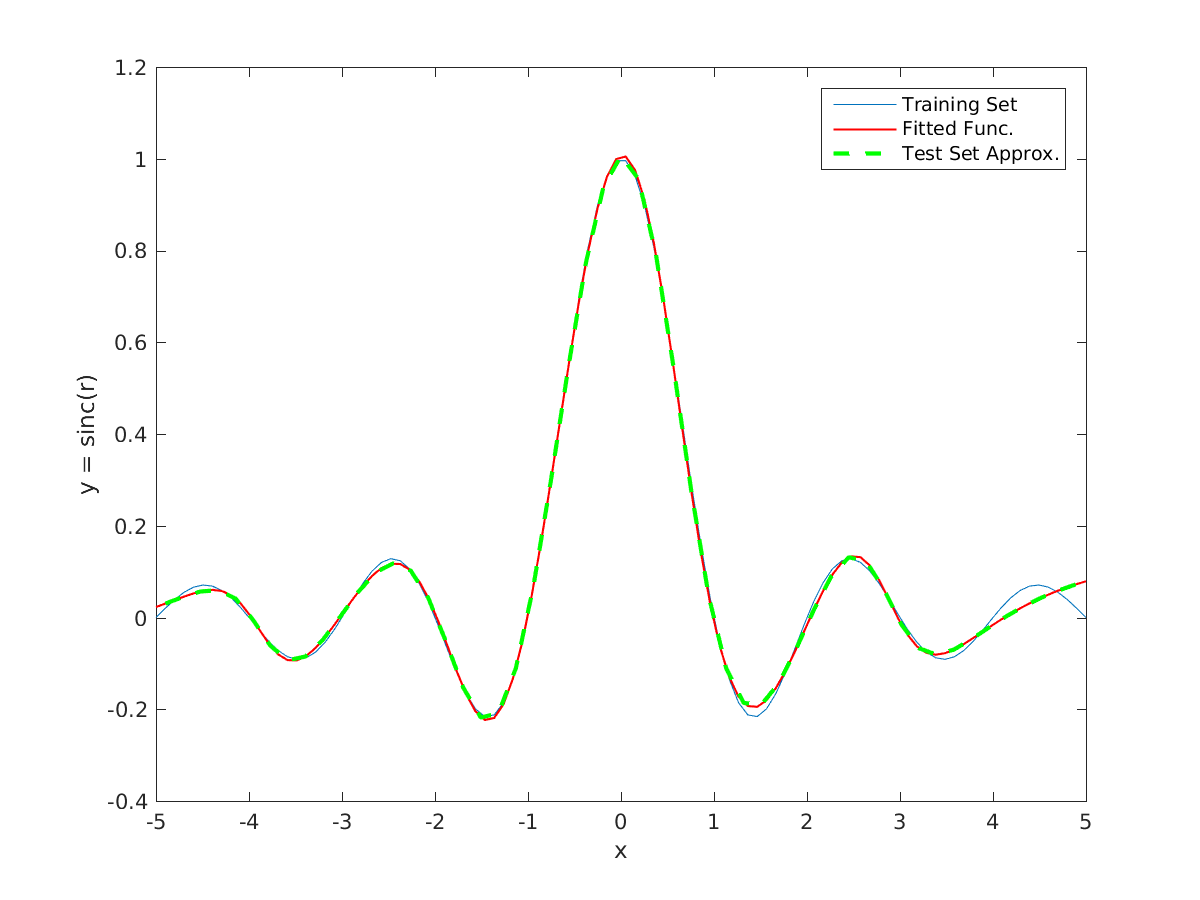
\includegraphics[width = \textwidth]{sinc1log.png}
		\caption{tanh activation}
	\end{subfigure}
	\begin{subfigure}[b]{0.5\textwidth}
		\centering
		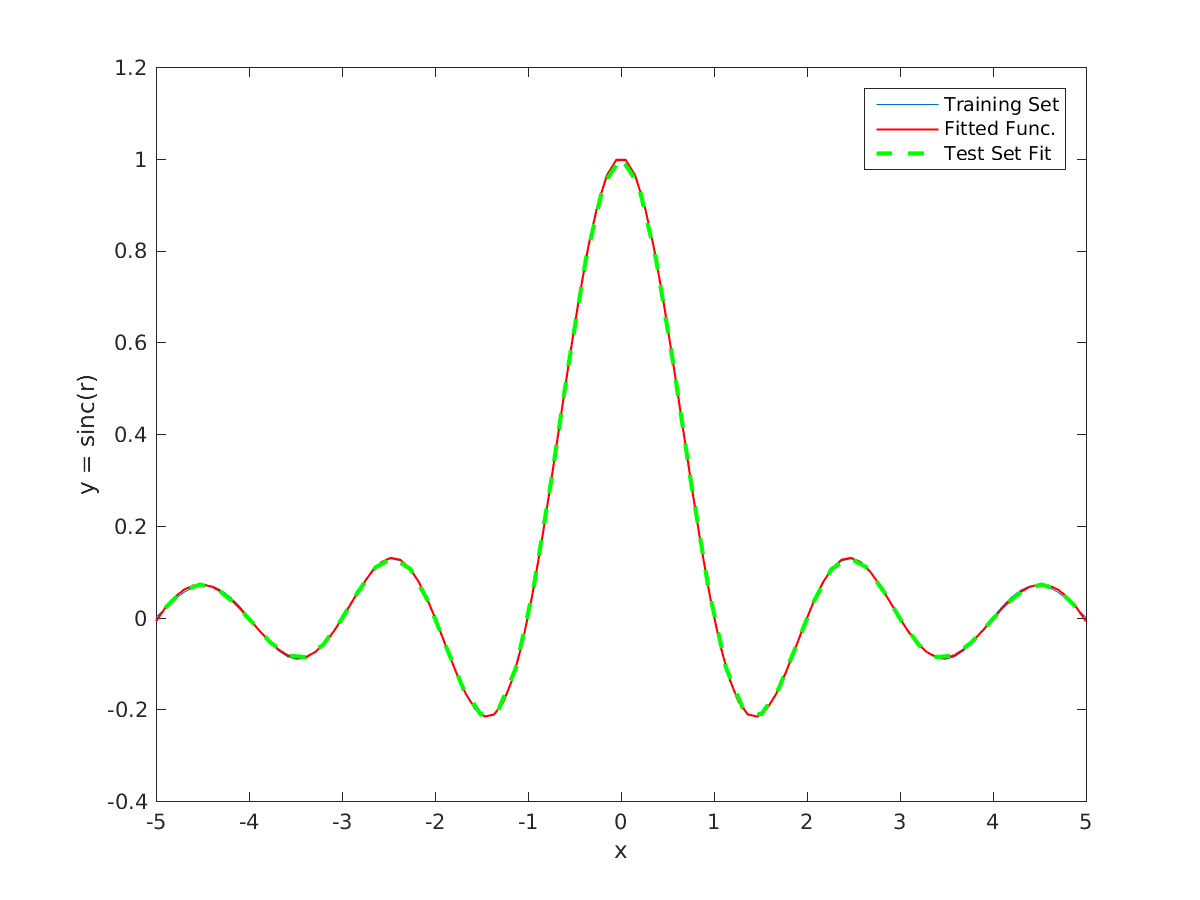
\includegraphics[width = \textwidth]{sinc1radbas.png}
		\caption{radial basis function (RBF)}
	\end{subfigure}
	\caption{Using an MLP with 5 hidden units to approximate sinc(x) on [-5,5].}
	\label{sinc1fit}
\end{figure}

The advantage of using a smaller number of neurons will become clearer for the cases with higher dimensionality.

\subsection*{Case m = 2}
Similar to the case for m=1, the aim is to use a neural network to train the \texttt{sinc} function for 2 dimensions. This function is also known as the mexican hat function. A plot of this function over the 2-dimensional interval $[-5,5]^2$ is given in figure \ref{sinc2}.

\begin{figure}[h]
\centering
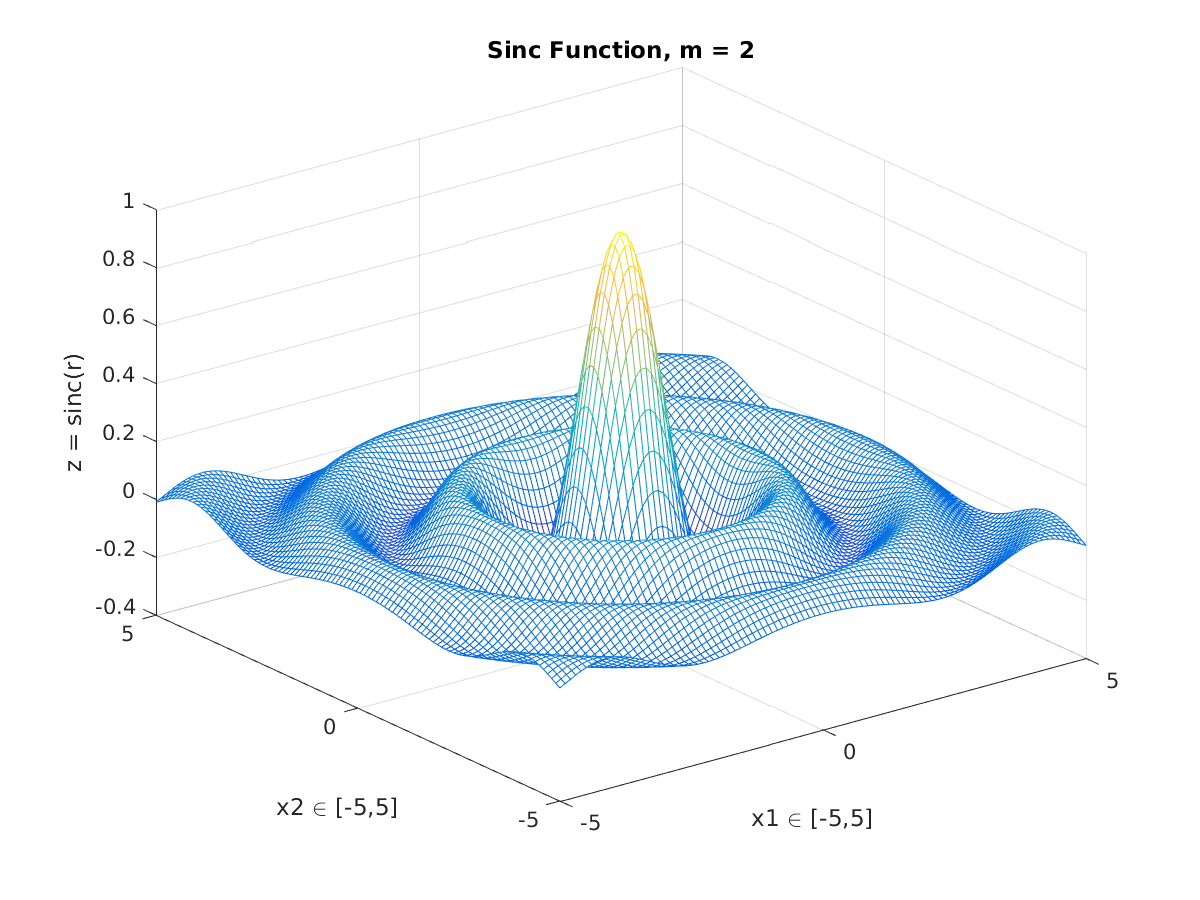
\includegraphics[width = 0.8\textwidth]{sinc2.png}
\caption{Mexican hat function on the 2-dimensional interval $[-5,5]^2$}
\label{sinc2}
\end{figure}

It is interesting to note, that in the 1-dimensional case, 100 points were used (training set) and there was a lesser amount of "empty space" in the plot. Comparing this to the 2-dimensional case, we see that there is a lot more "empty space" in 3-dimensions compared to 2-dimensions. If we take 100 equally spaced points for $x_1$ and $x_2$ $\in [-5,5]$, we get a grid of $100^2$ = 10,000 points in the training set. Thus, we observe that the number of cases $n$ has now increased from 100 to 10,000. Generally speaking, for an $m$-dimensional input space, the training set would contain 10$^m$ cases. This is known as the \emph{curse of dimensionality}.\\

We decide to go with the full training set with 10,000 points and use early stopping with a validation set consisting of 53 equally spaced points on [-4.9,4.9]. Thus, the validation set consists of 53$^2$ = 2809 points. Finally, a separate test set of 40$^2$=1600 points on [-4.8,4.8]$^2$ is created to evaluate the network performance and is not used at the time of training the network. The advantage of selecting these three sets is that they are mutually disjoint and hence, the network is evaluated on sets which are similar, but not the same as the training set. The activation function function used is the radial basis function which is selected due to it's advantage in using a smaller number of neurons. Levenberg-Marquadt algorithm is used to train the network due to it's fast convergence rate, however resilient backpropagation was tried and resulted in a poorer fit compared to the LM algorithm. The network was trained with 25 and 35 neurons. 

\begin{figure}[h]
	\begin{subfigure}{0.5\linewidth}
		\centering
		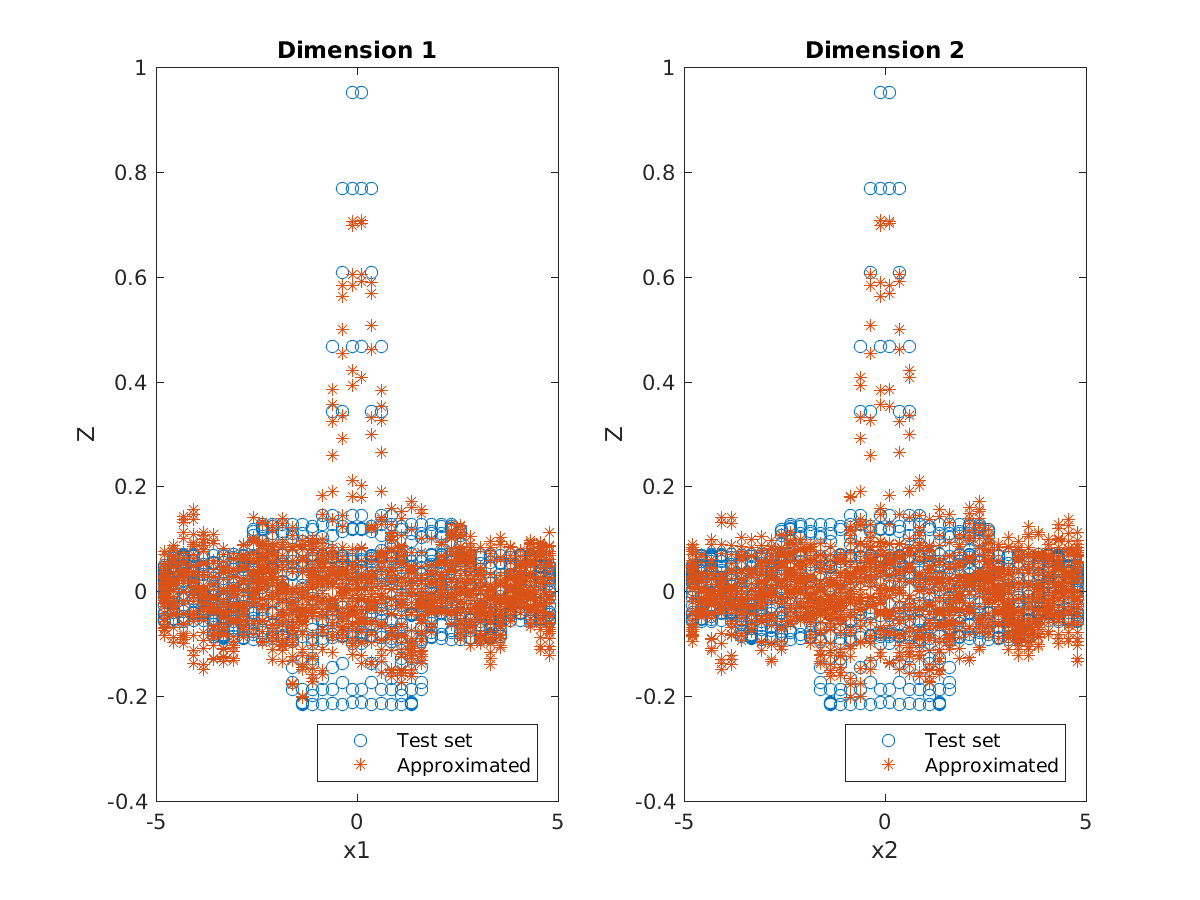
\includegraphics[width = \textwidth]{sinc2point25.png}
		\caption{25 neurons}
	\end{subfigure}
	\begin{subfigure}{0.5\linewidth}
		\centering
		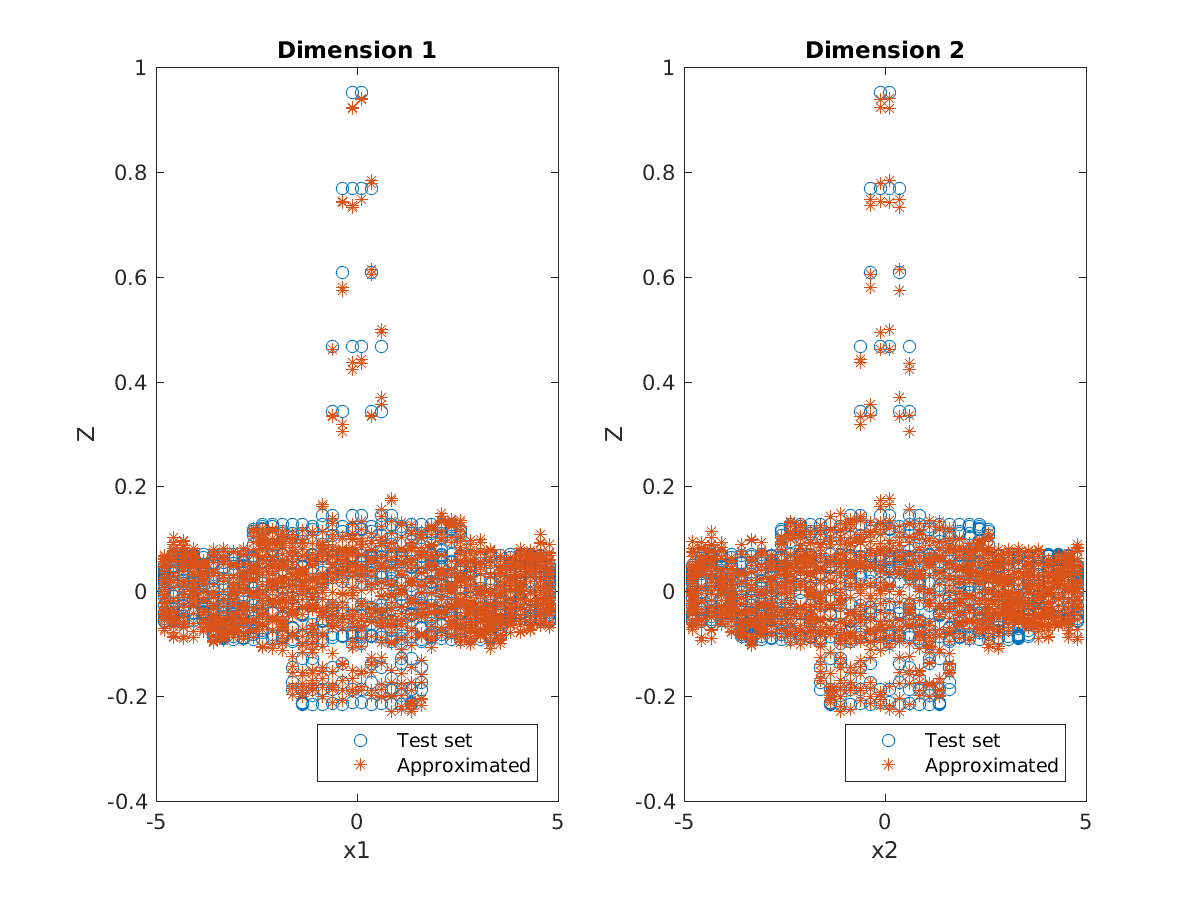
\includegraphics[width = \textwidth]{sinc2point35.png}
		\caption{35 neurons}
	\end{subfigure}
\caption{Mexican hat function in 2 dimensions. Plot of the test set with the approximated function on the test set. 25 and 35 neurons were tried.}
\label{sinc2fit}
\end{figure}

In figure \ref{sinc2fit}(a), we see that the network with 25 neurons is not able to adequately approximate the underlying function. The MSE on the test set  is 0.0039. In \ref{sinc2fit}(b) we see that the performance of the network with 35 neurons results in a rather good fit. The MSE was found to be 0.000494.

\subsection*{Case m = 5}
Now we arrive at the interesting part of the exercise: evaluating the \texttt{sinc} function in 5 dimensions. The first problem we run into is that the training and test sets cannot be chosen in a manner that was employed for the 1- and 2-dimensional cases. Selecting 100 equally points on a 5-dimensional grid, for example, will lead to $100^5$=10,000,000,000 observations which is simply too impractical. Furthermore, it would be challenging to visualize the approximated function due to the dimension being greater than 3. Thus, we compare the fitted models based on MSE on the training and test sets. 5 networks are trained with 100, 200, 300, 400 and 500 nodes in the hidden layer. Furthermore, we used the scaled conjugate gradient algorithm to train the network as it is suitable for large scale problems as it does not store large matrices in memory. Training set was chosen to be 15 equally spaced points on the $[-5,5]^5$ interval which results in $15^5$ = 759375 cases used to train the network. A validation set of 10 equally spaced points was chosen on the $[-4.9,4.9]^5$ which resulted in 100000 cases in the validation set. Similarly, a test set of 10 equally spaced points was chosen on the $[-4.8,4.8]^5$ which resulted in 100000 cases in the test set. Early stopping was used to train the network, however, due to time constraints, we trained the network for 100 epochs and training was stopped whichever of these two occurred first. 

\begin{table}
\centering
\begin{tabular}{|c|c|c|}
\hline
Hidden units & Training Set & Test sets \\ 
\hline
100 & 	0.0014	& 0.0014 \\
\hline
200 & 				& 			\\
\hline
300 & 			& 			\\
\hline
400 & 			&	 \\
\hline
500	& 			&		\\
\hline
\end{tabular}
\caption{MSE of the network on the test set for the sinc function in 5 dimensions.}
\label{sinc5}
\end{table}

\section{Session 2}
\subsection{Santa Fe laser prediction}
This exercise involves time-series prediction. The data are generated by a chaotic laser (which is a nonlinear dynamical system) and 1000 points are available for training the model. 100 observations are available for assessing the prediction of the model, which are not used at the time of training the model. A plot of the training set and the test set are given in figure \ref{santafe}.\\

\begin{figure}[ht]
\begin{subfigure}[b]{0.5\textwidth}
\centering
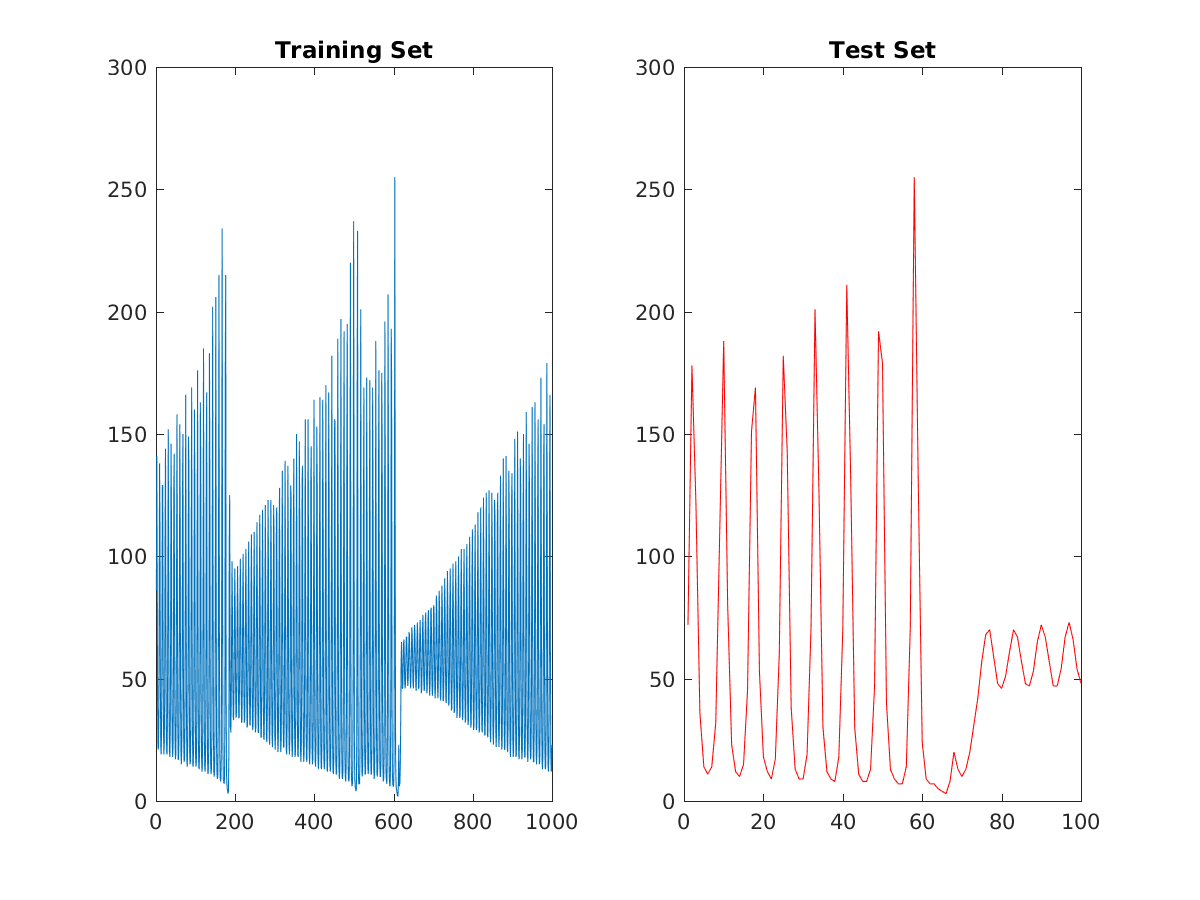
\includegraphics[width = \textwidth]{santafe.png}
\caption{Training and Holdout data}
\end{subfigure}
\begin{subfigure}[b]{0.5\textwidth}
	\centering
	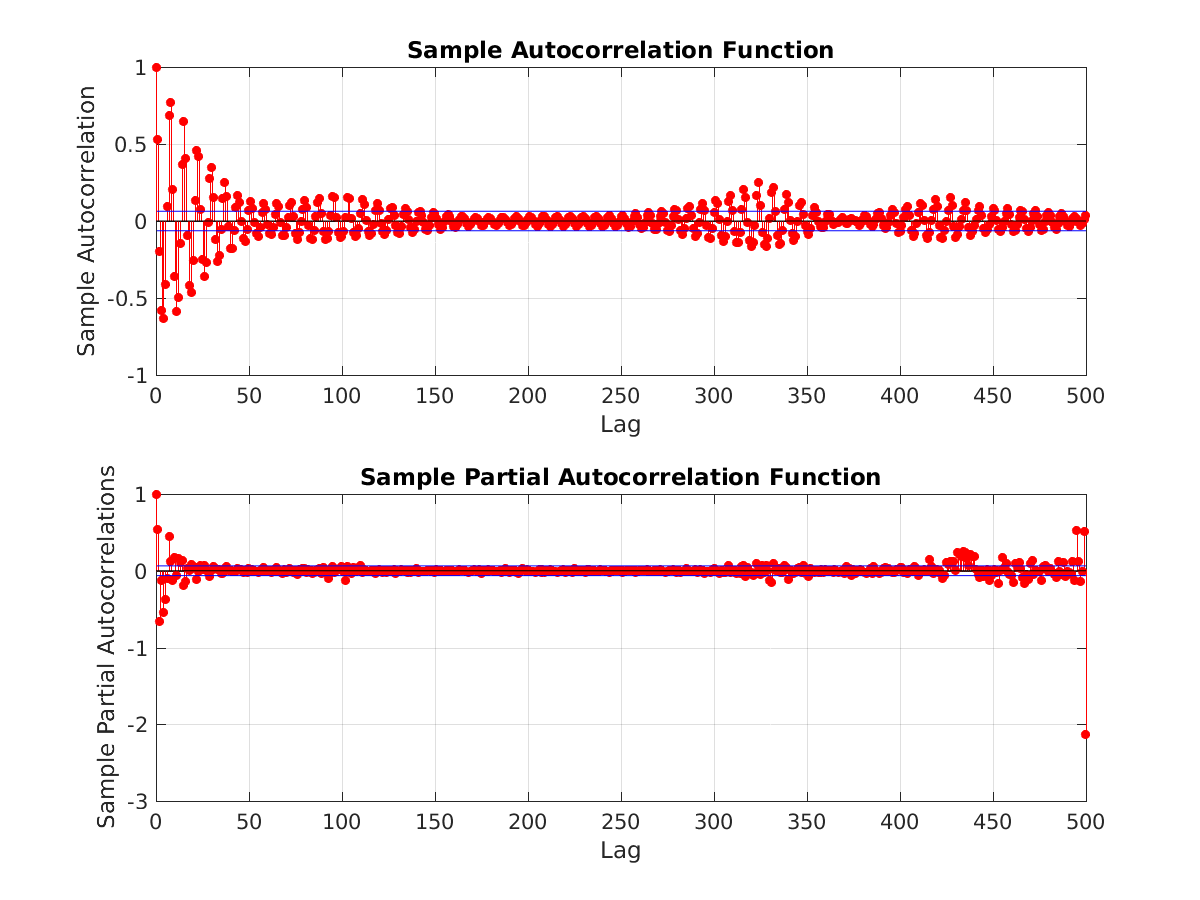
\includegraphics[width = \textwidth]{santafe_acf.png}
	\caption{Autocorrelation plots for the Santa Fe series.}
\end{subfigure}
\caption{Santa Fe data: series plotted on the left; with autocorrelation plots on the right.}
\label{santafe}
\end{figure}

We train an MLP with one hidden layer in feedforward mode using the training set. Symbolically, it can be expressed as $$\hat{y}_{k+1} = w^T\mathrm{tanh}(V[y_k; y_{k-1}; \ldots ; y_{k-p}] + \beta)$$ where $p$ is the lag of the series. The trained network was then used as a recurrent neural network to predict the next 100 iterations $$\hat{y}_{k+1} = w^T\mathrm{tanh}(V[\hat{y}_k; \hat{y}_{k-1}; \ldots ; \hat{y}_{k-p}] + \beta)$$ where the current predicted observation is fed back into the network to predict the next observation.\\

Different combinations of lags and neurons in the single hidden layer were tried and the scaled conjugate gradient algorithm was used for training the network with a regularization parameter of $10^{-6}$.  The cost function employed for training was the MAE (mean absolute error). The evaluation of the network on the test set was done using the MAE (mean absolute error). The (partial) autocorrelation plot of the original series is given in figure \ref{santafe}. We can see from the PACF that the first 16 spikes are significant, thus, we can start with a NAR model with 16 lags. For brevity, we restrict ourselves to trying 16, 25, 40 and 60 lags and use (number of lags)/2 as the number of hidden layer neurons. Using regularization should keep the weights of the network from getting too big. Alas, there appear to only be rules of thumb for choosing the number of hidden units and no concrete method.\\ 

The data were divided first in blocks (80\% for training and 20\% for validation), however, random division of the dataset into training and validation resulted in better performance. Random division does not seem particularly sensible a method with time series data as the observations are not IID samples but are correlated with each other. Destroying this correlation structure is akin to then throwing the baby out with the bathwater. After selecting the number of lags, we then retrained the network by manually selecting the training and the test set indices and assessing the effectiveness of the network at approximating the target series with the holdout data. The approximated function from the fit are shown in figure \ref{lag}.\\

\begin{figure}[ht]
	\begin{subfigure}[b]{0.5\textwidth}
		\centering
		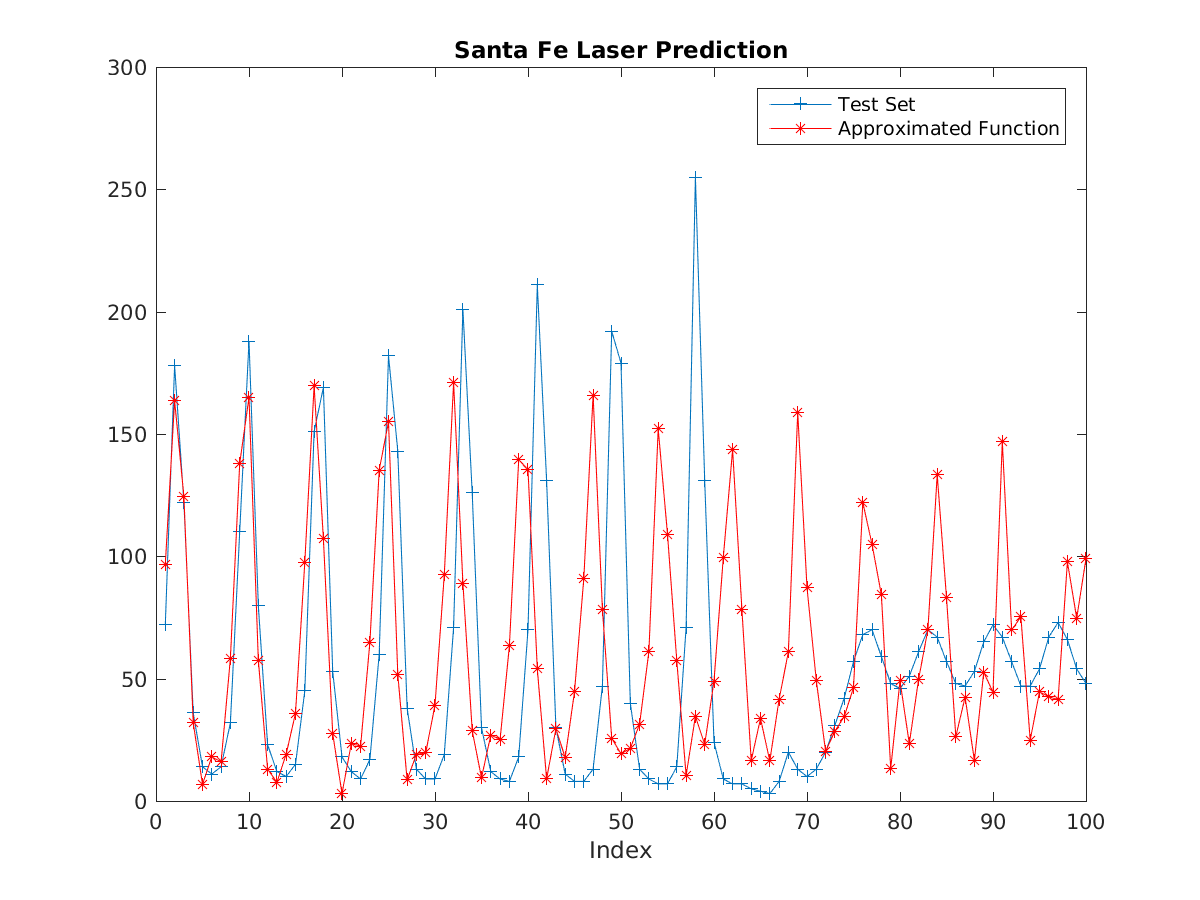
\includegraphics[width = \textwidth]{santafe_pred16.png}
		\caption{16 lags (delays)}
	\end{subfigure}
	\begin{subfigure}[b]{0.5\textwidth}
		\centering
		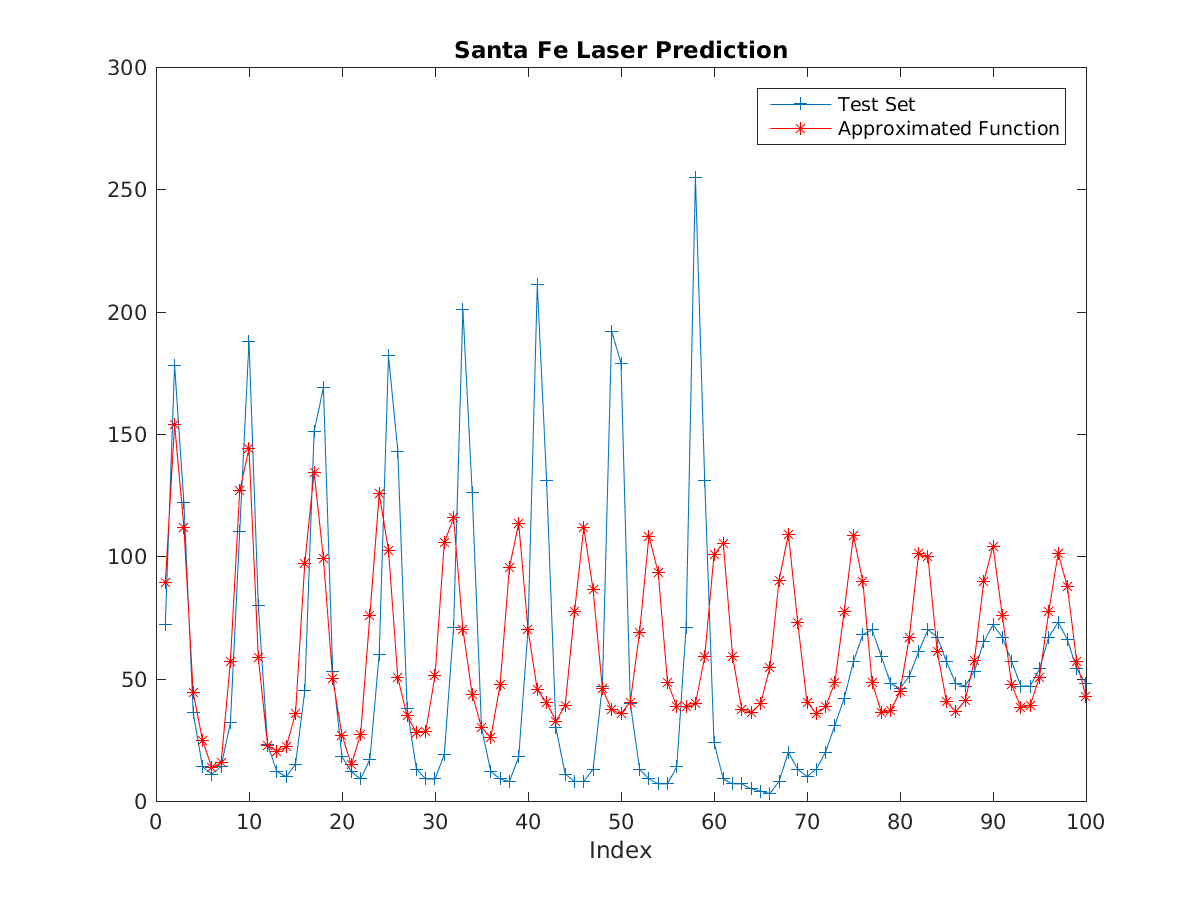
\includegraphics[width = \textwidth]{santafe_pred25.png}
		\caption{25 lags (delays)}
	\end{subfigure}
	% leave a line
	
	\begin{subfigure}[b]{0.5\textwidth}
		\centering
		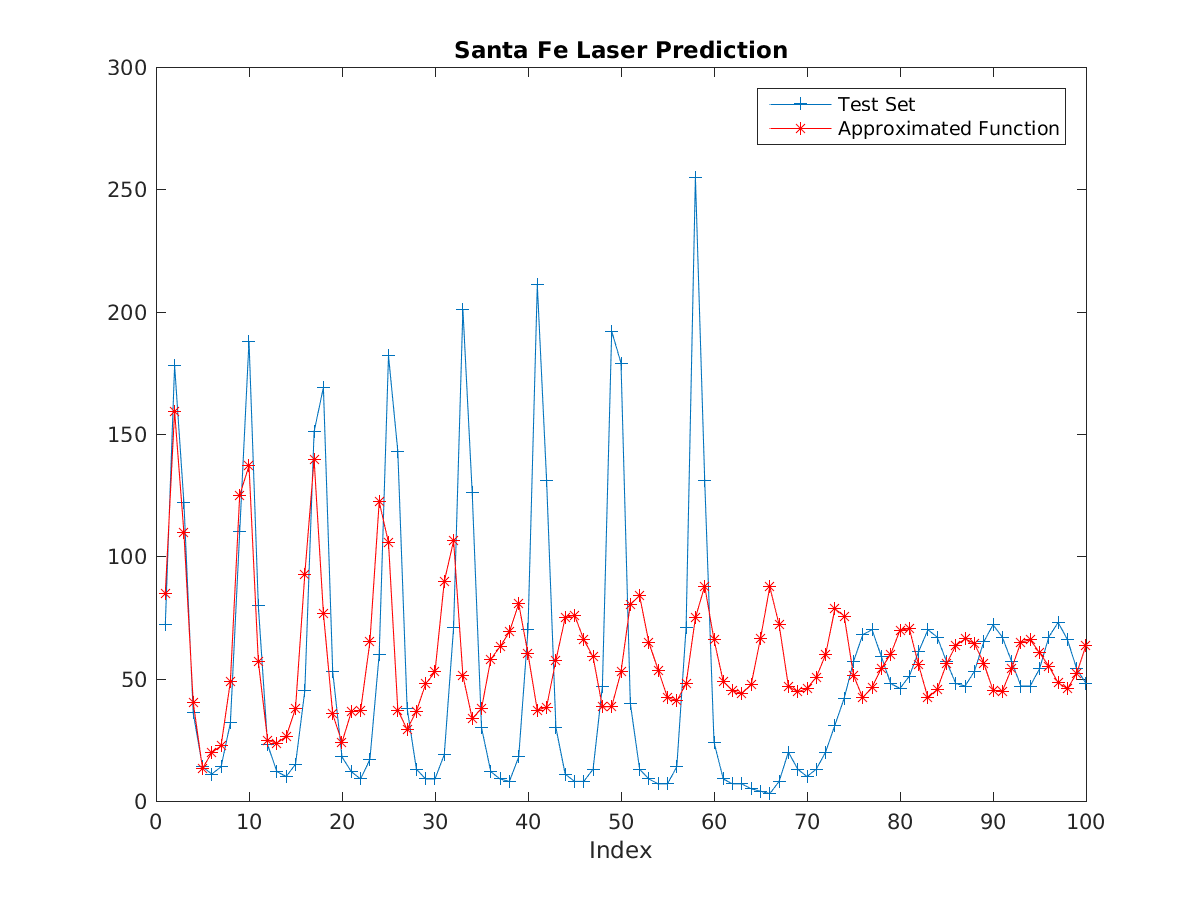
\includegraphics[width = \textwidth]{santafe_pred40.png}
		\caption{40 lags (delays)}
	\end{subfigure}
	\begin{subfigure}[b]{0.5\textwidth}
		\centering
		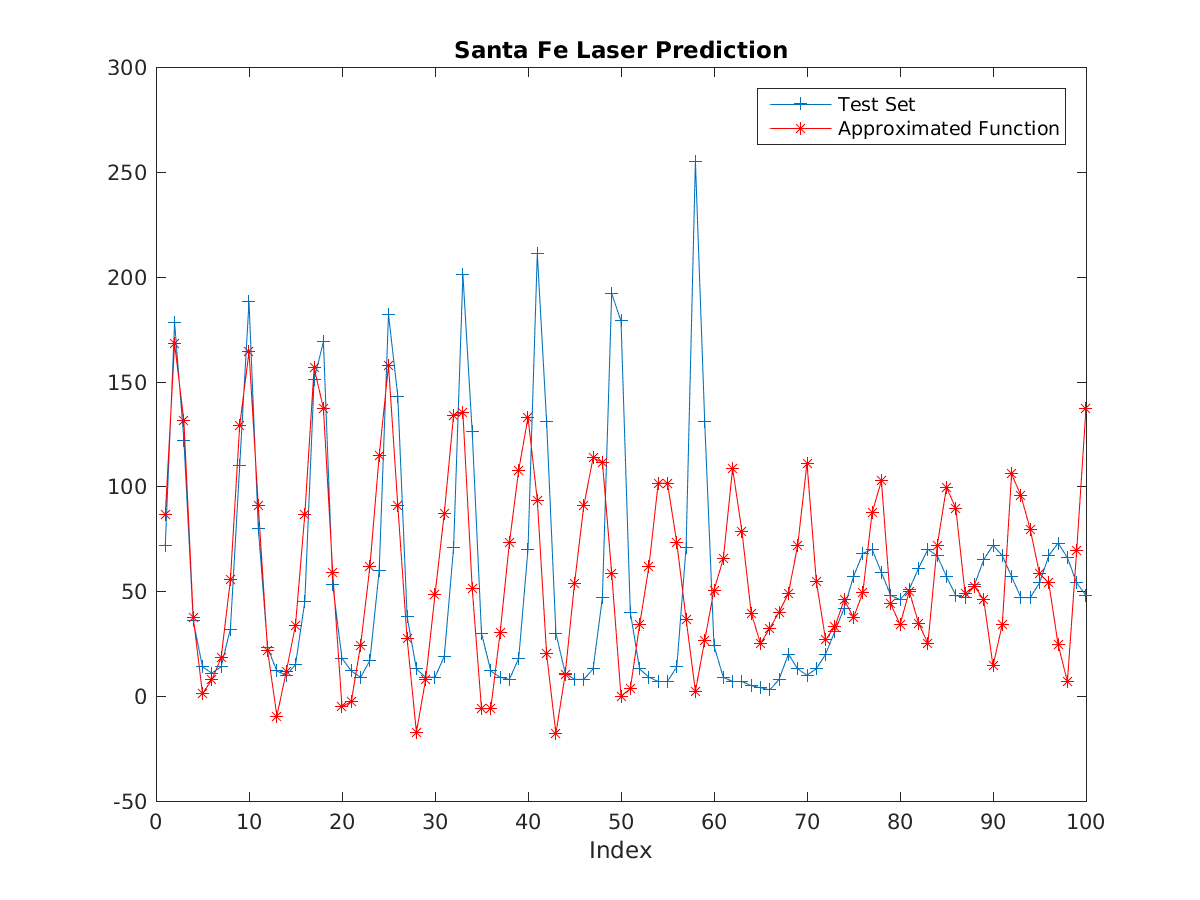
\includegraphics[width = \textwidth]{santafe_pred60.png}
		\caption{60 lags (delays)}
	\end{subfigure}
\caption{Santa Fe: approximated function fit to the holdout set. 4 different lag values were considered (16, 25, 40, 60) and hidden units = (lags/2). Regularization parameter is taken to be $10^{-6}$.}
\label{lag}
\end{figure}

Based on these graphs, we pick the 16 lags case and the 60 lags case for the manual training/validation set division and compare the accuracy of the approximated function. We took the first 80 observation (1:80, 101:180, $\ldots$, 901:980) as the training set and the last 20 as validation set (81:100, 181:200, $\ldots$, 981:1000). Other combinations could be tried as well, however manually specifying training and validation sets can lead to loss of important information from the training series. Splitting time series into training and validation sets is a non-trivial task, and one usually learns in a time series course to fit a model by training the model based on minimizing the one-step ahead prediction errors. A plot of the approximated function for 16 and 60 lags is given in figure \ref{manual}.

\begin{figure}[ht]
	\begin{subfigure}[b]{0.5\textwidth}
	\centering
	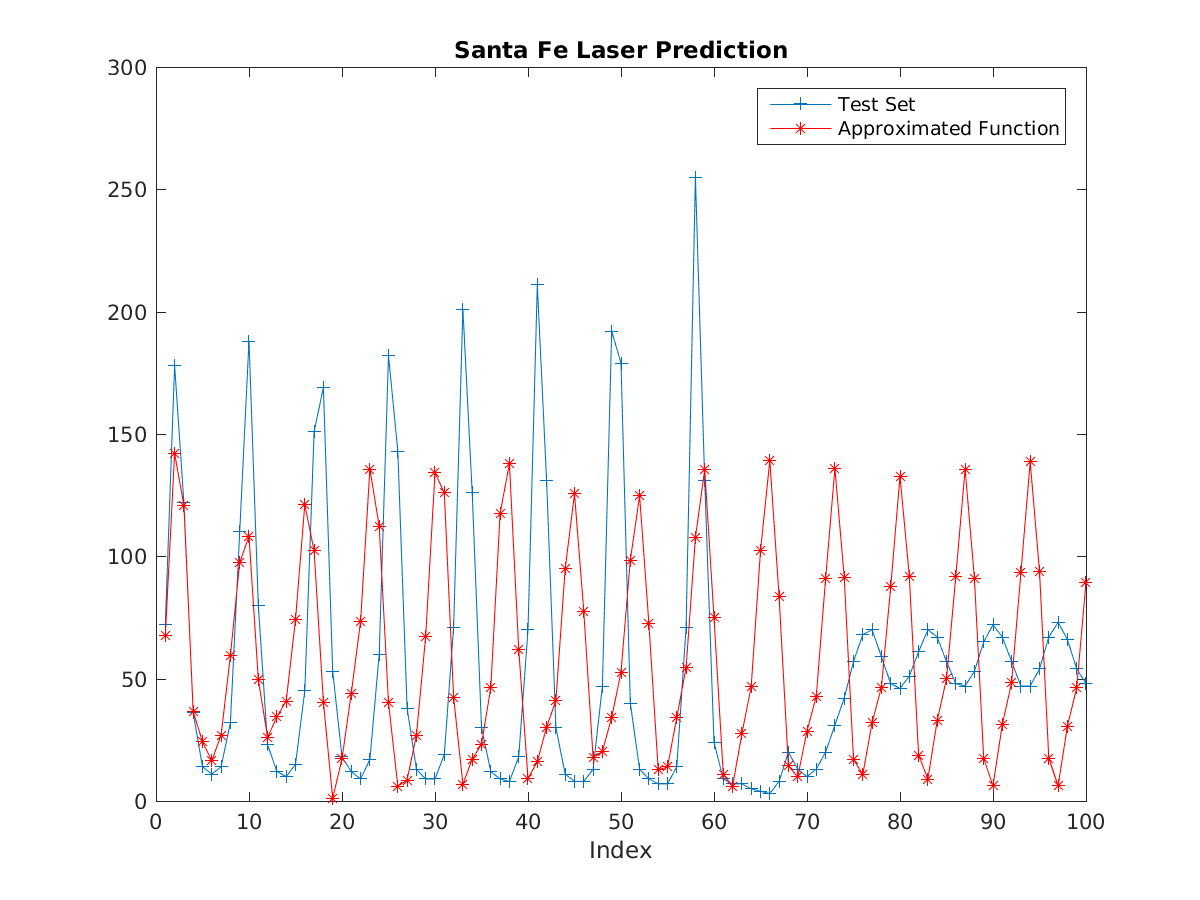
\includegraphics[width = \textwidth]{manual_lag16.png}
	\caption{16 lags}
	\end{subfigure}
	\begin{subfigure}[b]{0.5\textwidth}
	\centering
	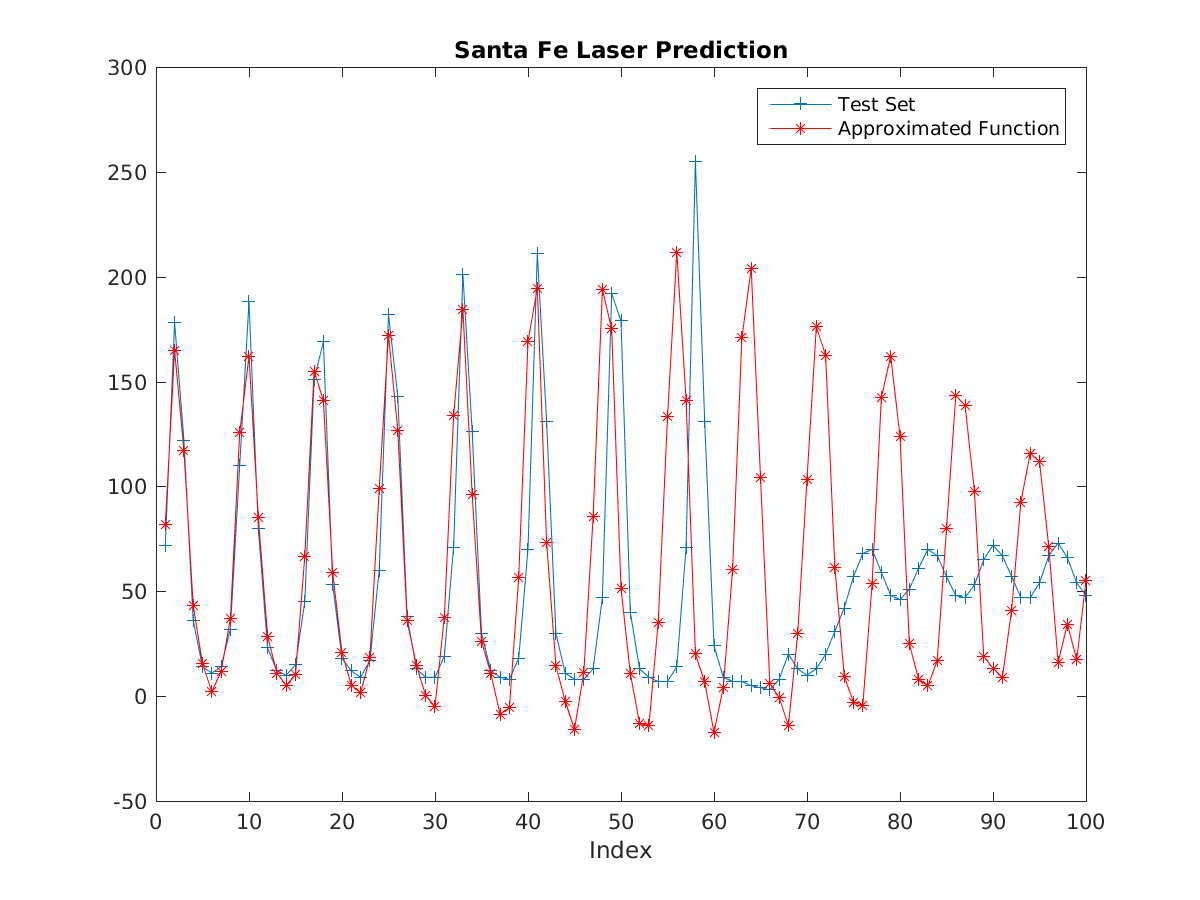
\includegraphics[width = \textwidth]{manual_lag60.png}
	\caption{60 lags}
	\end{subfigure}
\caption{Santa Fe dataset: Manual division of the data into training and validation sets and using 16 and 60 lags.}
\label{manual}
\end{figure}

\subsection{Alphabet recognition demo: appcr1}

This demo uses a neural network (MLP) for a classification task, namely alphabet recognition. A feedforward network with a 25 hidden units in a single hidden layer and 26 nodes in the output layer (for the 26 different characters in the alphabet) was used for training the network. Two different sets of inputs (shown in figure \ref{char} were used to train two different networks (noiseless: net1; noisy: net2), both possessing the same architecture (figure \ref{charnet}). \\

\begin{figure}[ht]
\begin{subfigure}{0.5\textwidth}
		\centering
		
\includegraphics[width = 0.8\textwidth]{d_noiseless.png}
		\caption{Noiseless Case}
	\end{subfigure}
	\begin{subfigure}{0.5\textwidth}
		\centering
		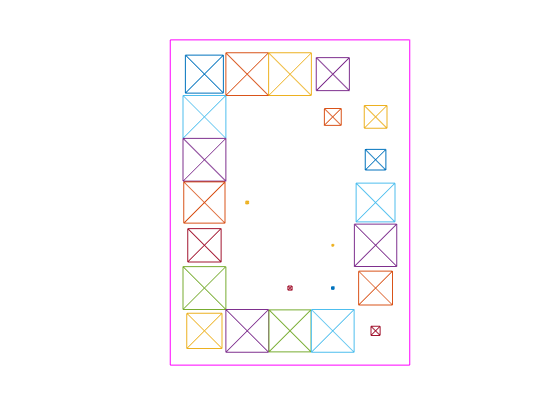
\includegraphics[width = 0.8\textwidth]{d_noise.png}
		\caption{Noisy Case}
	\end{subfigure}
\caption{Alphabet recognition: Letter D without noise and with noise}
\label{char}
\end{figure}

The input data presented to net1 contains no noise. In the second case, the input data presented to net2 contains a noisy version (added noise from a $N(0,0.2^2)$) of the letter D. Thus, it seems reasonable to expect net2 to perform well on both the noiseless and noisy cases compared to net1, but net1 to perform worse on noisy data than net2's performance on noiseless data.\\

\begin{figure}[ht]
\centering
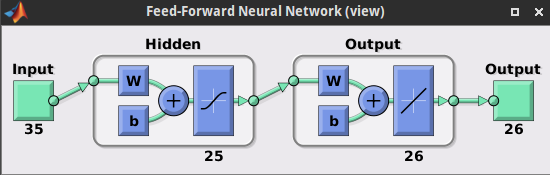
\includegraphics[width = 0.5\textwidth]{22_net.png}
\caption{Architecture of the network used for alphabet recognition demo \emph{appcr1}}
\label{charnet}
\end{figure}

The dataset is created as follows: each image is broken into a 5x7 bitmap of a letter. These 35 pixel values are added to a matrix with 26 columns. Thus, it results in a 35x26 matrix, with each column representing a letter of the alphabet, and each row corresponds to a pixel of the image. In the noiseless data, the pixels are either 0 or 1. However, in the noisy case, some of the pixels are now not exactly 0 or 1 but have some added noise. The target matrix is a 26x26 identity matrix which maps each alphabet to a class. Thus, the fifth diagonal entry will indicate the letter E, etc. Finally, the networks are tested with 20 different levels of noise ($0.05, 0.1, 0.15, \ldots, 1.0$). A plot comparing the performances of the two networks is presented in figure \ref{charerr}.\\

\begin{figure}[ht]
\centering
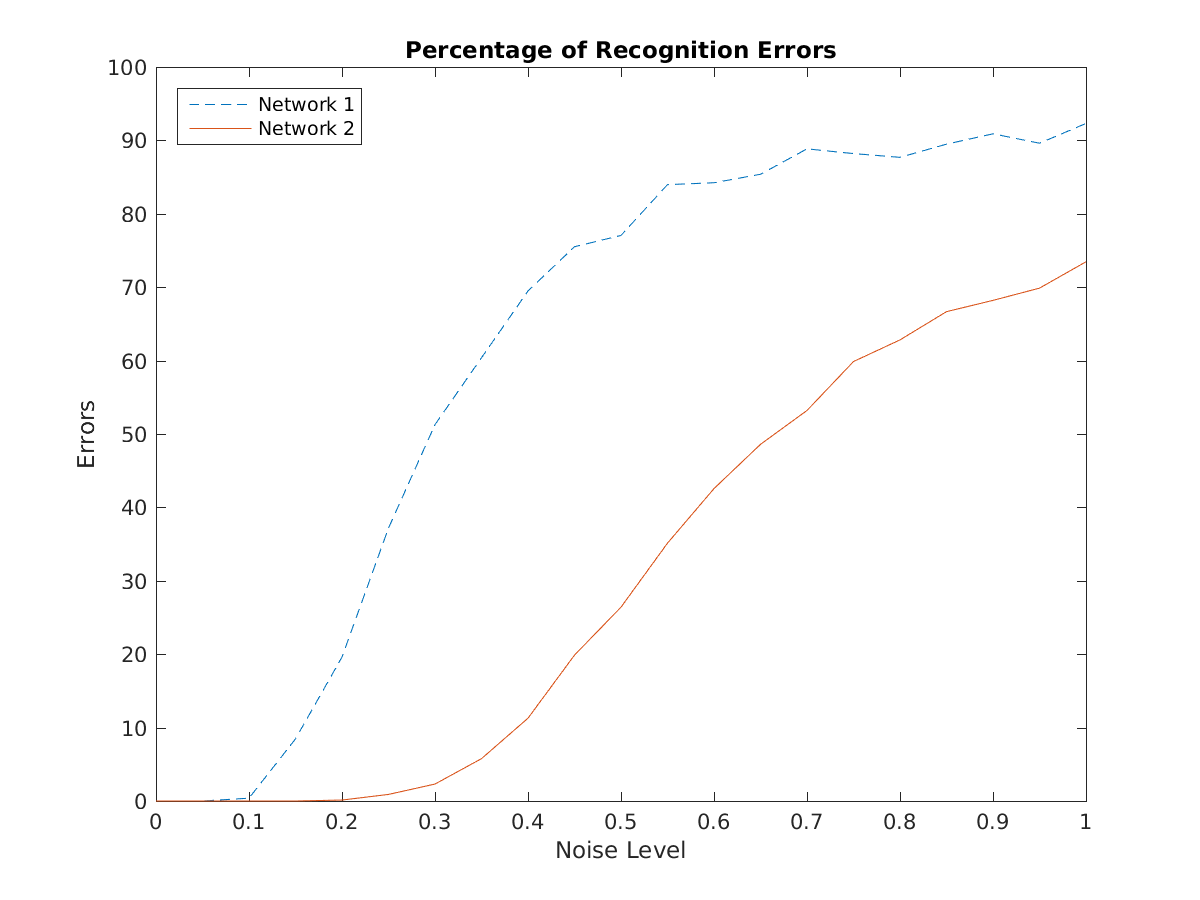
\includegraphics[width = 0.6\textwidth]{char_err.png}
\caption{Character recognition: plot comparing the classification performance of the two networks on inputs with 20 different levels of noise ($0.05, 0.1, 0.15, \ldots, 1.0$). Network 2 naturally performs better than network 1 due to being trained on noisy data.}
\label{charerr}
\end{figure}

Thus, we see from figure \ref{charerr} that net2 has overall much better performance than net1. Net1 is able to handle noise upto 0.2 with an error rate less than 20\%. Net2, on the other hand, has less than 20\% error for noise upto $\sigma$=0.5 and has negligible errors for $\sigma \leq 0.25$ (as the network was trained on data with noise parameter 0.2). Net1 has negligible errors for $\sigma \leq 0.1$. It is a little surprising to see that despite being trained on noiseless data, network 1 is robust to a small amount of noise. 

\subsection{Pima Indians diabetes (classification problem)}
This problem is a classification problem, where a neural network will be trained as a classifier. We consider the UCI Pima Indians Diabetes dataset, which contains 768 records of female Pima Indians on 8 features. Further, the target variable has two levels: -1 (no diabetes) and 1 (diabetes). Next, we use a multilayer perceptron with one hidden layer for the classification problem at hand by considering it as a regression problem where the network is trained in the same way as regression. However, the values predicted after training the network $\notin \{0,1\}$, but $\in [0,1]$. Thus, we use the $Y=0.5$ as the decision rule, where $Y>0.5$ is classified as 1, and $Y<0.5$ is classified as 0.\\

The features were linearly scaled before training, and the target variable was scaled to \{0,1\} from \{-1,1\}. We used the scaled conjugate gradient algorithm with cross-entropy as the loss function. Early stopping was used instead of regularization. Four separate networks were trained with 2, 5, 8 and 10 neurons by using 60\% of the observations in the training set, and 20\% for the validation and test sets respectively. The cross-entropy errors and the corresponding confusion matrices are presented below.\\

From figure \ref{pima}, we see that the performance for all the networks is very similar. Each of the networks were trained multiple times (not included here) to assess the sensitivity of the classifier to random initial weights. Across all the different runs, the classifier was able to correctly classify somewhere between 70-80\% of the observations in the test set. This indicates that the training algorithms keep getting stuck in local minima and is rather sensitive to random data division as well as the initial weights for the training algorithms. Since all the networks with different neurons give similar results, we can select the network with 2 or 5 neurons in the hidden layers for parsimony. To reduce the sensitivity of the model to initial weights, one can apply 10-fold cross-validation and average the weights from these models for prediction. Furthermore, since the division of the data into the training/validation/test sets were random, this could be a factor in the (relatively) large differences between different models (with the same number of neurons). The cross-validation method should lead to a robust network in this case as well.\\

\begin{table}[H]
\centering
\begin{tabular}{lcccc}
\hline
Neurons & 2 & 5 & 8 & 10\\
\hline
Error & 0.4618 & 0.4796 & 0.4776 & 0.4639 \\
\hline
\end{tabular}
\caption{Pima diabetes: Cross-entropy error from training the network with different number of neurons for the Pima Indians diabetes classification problem.}
\label{cross}
\end{table}

\begin{figure}[H]
	\begin{subfigure}[b]{0.5\textwidth}
		\centering
		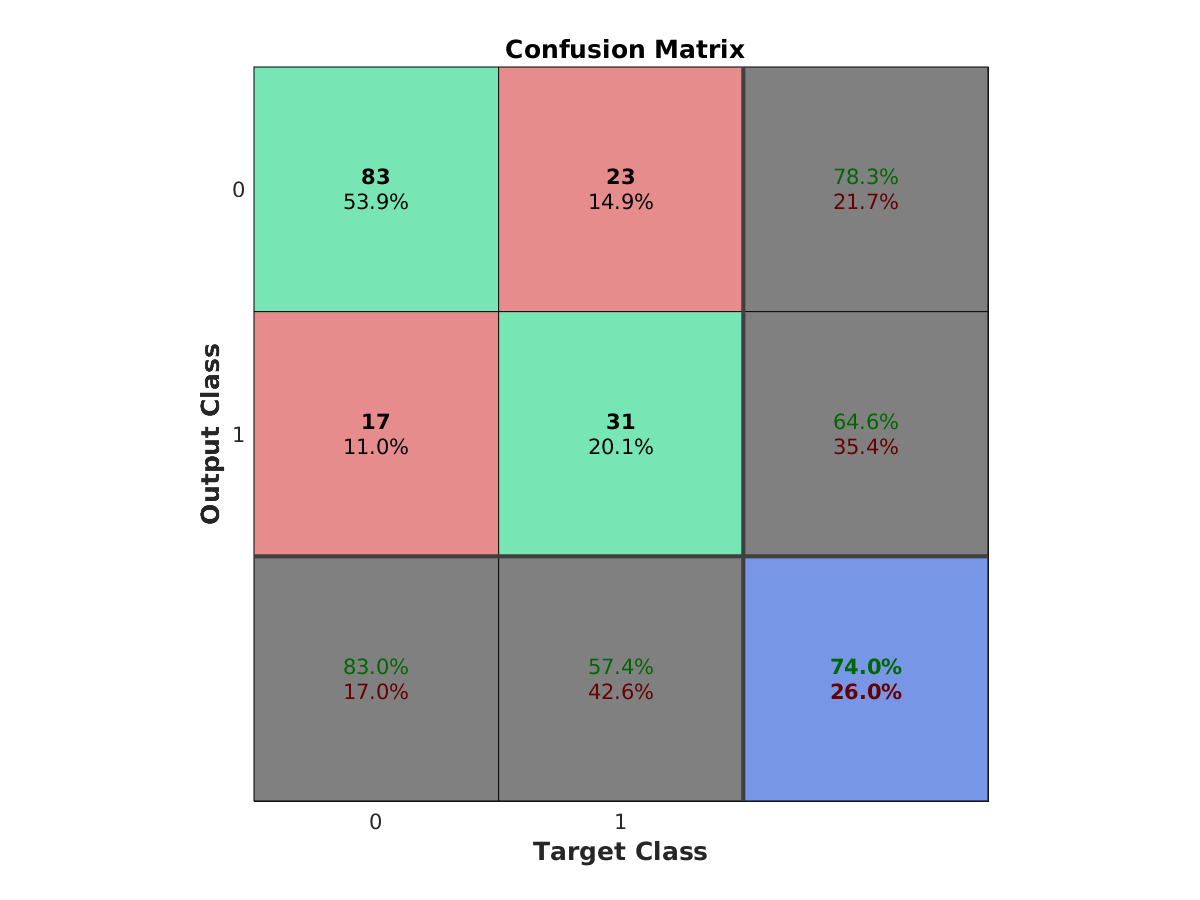
\includegraphics[scale = 0.4]{pima_confusion_2.png}
		\caption{2 Neurons}
	\end{subfigure}
	\begin{subfigure}[b]{0.5\textwidth}
		\centering
		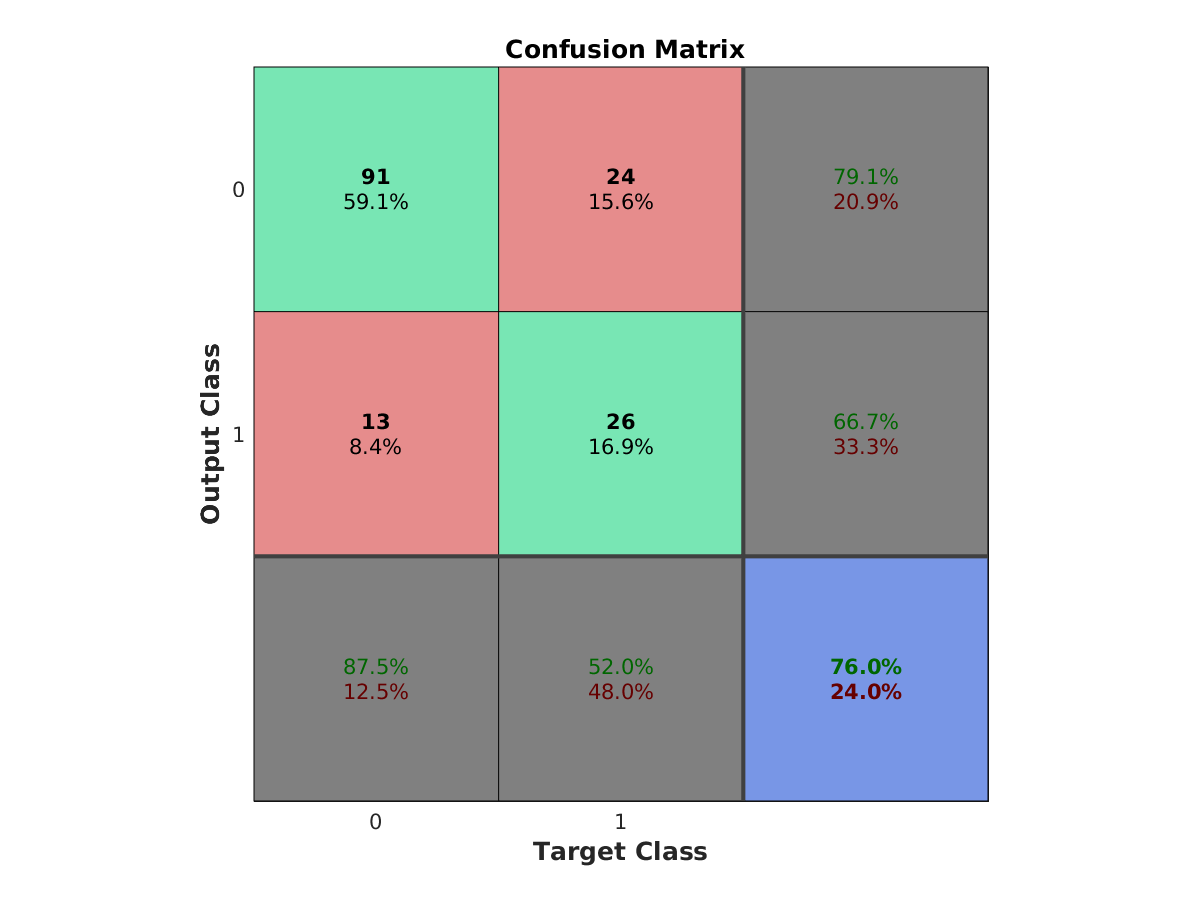
\includegraphics[scale = 0.4]{pima_confusion_5.png}
		\caption{5 Neurons}
	\end{subfigure}
	% leave a line to create a 2x2 grid
	
	\begin{subfigure}[b]{0.5\textwidth}
		\centering
		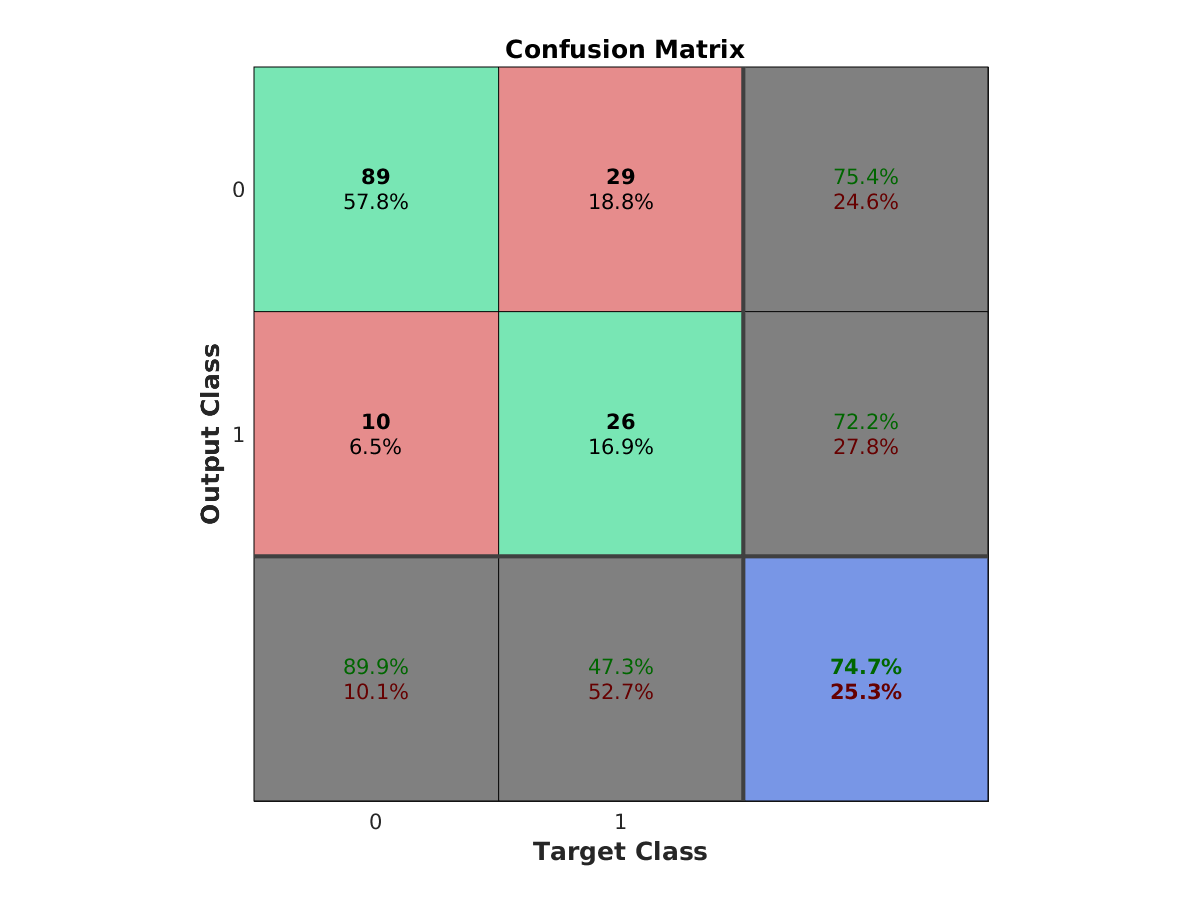
\includegraphics[scale = 0.4]{pima_confusion_8.png}
		\caption{8 Neurons}
	\end{subfigure}
	\begin{subfigure}[b]{0.5\textwidth}
		\centering
		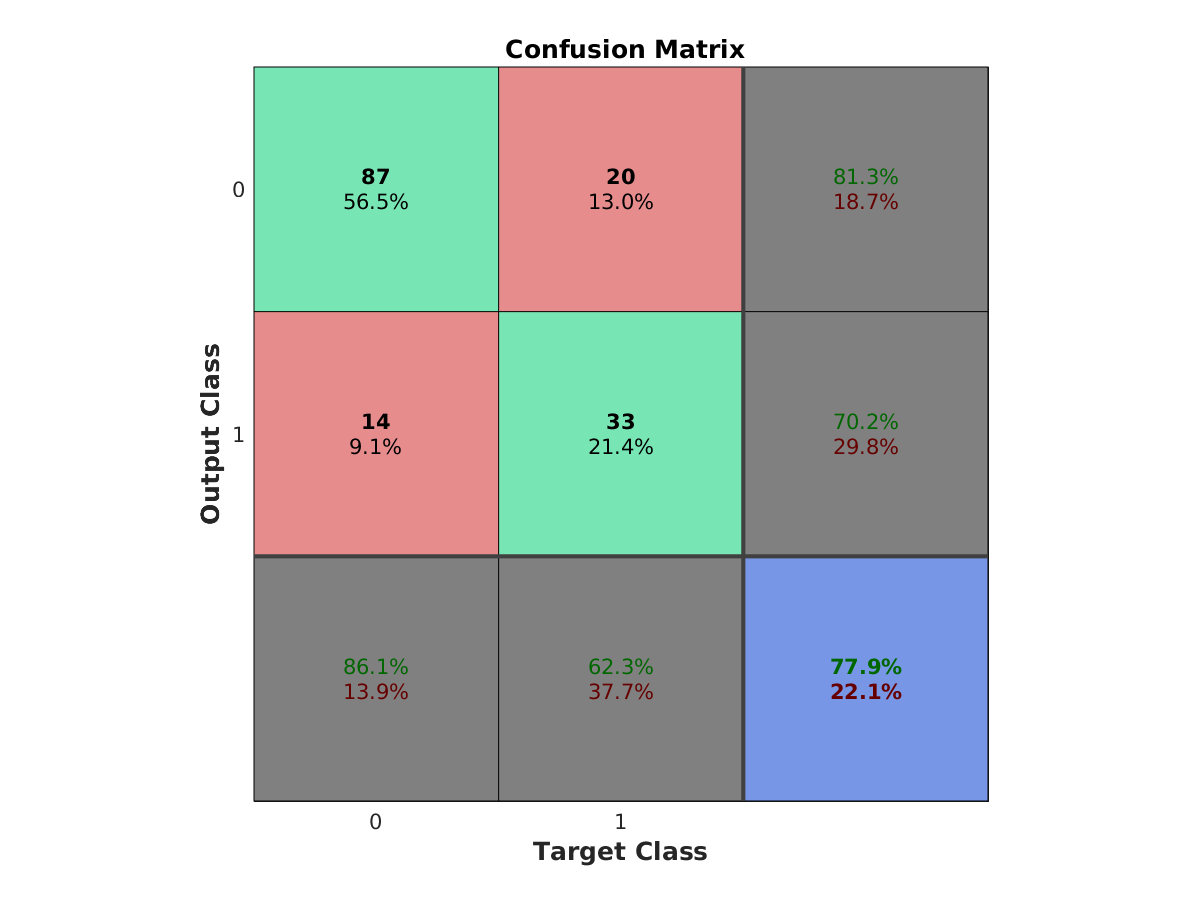
\includegraphics[scale = 0.4]{pima_confusion_10.png}
		\caption{10 Neurons}
	\end{subfigure}
\caption{PIMA Classification: confusion matrix with 2, 5, 8 and 10 neurons in the hidden layer}
\label{pima}
\end{figure}

\section{Session 3}
\subsection{Dimensionality reduction: Principal Component Analysis}

This dataset contains 21 measurements (inputs) on 264 samples. There are three target variables (namely LDL, VLDL and HDL) with multiple levels. First, we use all the 21 input variables for training the network and compare the performance of the Levenberg-Marquadt and the Bayesian regularization algorithms on the test set. Then, we transform the original input space using PCA and reduce the dimension of the input space from 21-dimensions to a 4-dimensional space (i.e., keeping the first 4 principal components).\\

Both the inputs and outputs were normalized before training the network. This is done to ensure that all the variables are on the same scale, and hence importance is not given to any particular variable(s) by the principal components simply due to differences in scale. The network was trained using 5 hidden units (with tanh activation function) in a single hidden layer with 3 nodes (with linear activation function) in the output layer. Early stopping rule was applied by using an independent validation set where the performance of the neural network was assessed on this validation set and the training was not stopped as long as the performance of the network on this validation set kept decreasing.\\

\begin{table}[h]
	\begin{minipage}{0.5\linewidth}
		\centering
		\begin{tabular}{ccc}
 & Training set & Test set \\
\hline
\thead{Early \\ Stopping} & 0.3036 & 0.2626 \\
\thead{Bayesian \\ Regularization} & 0.3103 & 0.2589 \\
\hline
		\end{tabular}
		\caption*{(a) 21 inputs}
	\end{minipage}
	\begin{minipage}{0.5\linewidth}
		\centering
		\begin{tabular}{ccc}
& Training set & Test set \\
\hline
\thead{Early \\ Stopping} & 0.3908 & 0.2605 \\
\thead{Bayesian \\ Regularization} & 0.3436 & 0.2704 \\
\hline
		\end{tabular}
		\caption*{(b) 4 inputs}
	\end{minipage}
\caption{PCA: Performance of the network with 21 inputs compared to 4 inputs and using Levenberg-Marquadt algorithm with early stopping and with Bayesian regularization}
\label{pca}
\end{table}

From table \ref{pca}, we see that the performances of the two networks on the test set are very similar. The effective number of parameters $\gamma$ with 21 inputs is 46 (out of 128), and with 4 inputs is 36 (out of 43). This indicates that a lot of the parameters are largely redundant. Additionally, since the MSE on the test set is very similar to the MSE on the training set in all cases, this means that the network has good generalization ability as it performs similarly on the test data that was not used to train the network. When the early stopping rule was used, the performance of the network was assessed on a separate validation set. However, in case of Bayesian regularization, the training and validation sets were used to train the model and the performance was assessed on the test set.\\

Since the network with reduced input has a much smaller number of less relevant parameters, we can select the model with the PCA transformed inputs. As an aside, if interpretation of the model were the aim, then the model with initial inputs would most likely be selected unless the 4 principal components were easily interpretable. However, since neural networks can be "blackboxes", so to speak, we decide to go with the model with reduced inputs. Lastly, we select the model with Bayesian regularization based on the principle of parsimony in that the regularization aims at keeping the interconnection weight values small. 

\subsection{Input selection: Automatic Relevance Detection}
\subsubsection*{Demo: demard}

This demo shows how a MLP can be used for automatic relevance detection on the input variables to determine which variables are relevant for the target variable. The input variables are $X_1$ $\mytilde$ $\mathbb{U}(0,1)$ with small amount of Gaussian noise, $X_2$ a copy of $X_1$ with higher amount of Gaussian noise and $X_3$ is an IID sample from a Gaussian distribution. The target variable t = sin(2$\pi x_1$) + $\varepsilon$, where $\varepsilon$ is Gaussian noise. Thus, $X_1$ should be really relevant for determining the target variable, $X_2$ less relevant and $X_3$ irrelevant out of these three. The function is displayed in figure \ref{demard}.

\begin{figure}[H]
\centering
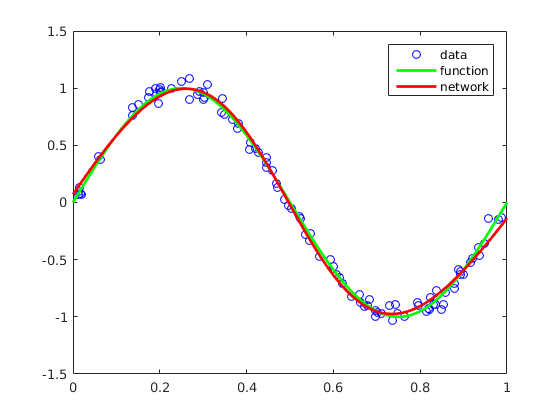
\includegraphics[width = 0.5\textwidth]{demard.png}
\caption{ARD Demo: data generating function (green) and approximated function (red)}
\label{demard}
\end{figure}

The prior distribution over the weights is given by the ARD Gaussian prior with a separate hyper-parameter for the group of weights associated with each input. The network is trained by error minimization using scaled conjugate gradient function SCG. There are two cycles of training, and at the end of each cycle the hyper-parameters are re-estimated using the evidence.\\

This results in the following values for the $\alpha_i$'s, i.e.\, the hyperparameters for the corresponding input to hidden unit weights: $\alpha_1$ = 0.21013, $\alpha_2$ = 1.70906, and $\alpha_3$ = 3154.38379 after the first training cycle. After the second training cycle, the hyperparameter values corresponding to the three inputs $x_1$, $x_2$ and $x_3$ are $\alpha_1$ = 0.17555, $\alpha_2$ = 21.07742 and $\alpha_3$ = 153182.97363.\\
 
Since each alpha corresponds to an inverse variance, we see that the posterior variance for weights associated with input x1 is large, that of x2 has an intermediate value and the variance of weights associated with x3 is small. The corresponding weight values are given below:

\begin{align*}
x_1: \quad -3.18149 \quad 1.10024 \\
x_2: \quad -0.24288 \quad 0.05027 \\
x_3: \quad  0.00119 \quad -0.00048
\end{align*} 
 
We see that the network is giving greatest emphasis to x1 and least emphasis to x3, with intermediate emphasis on x2. Since the target t is statistically independent of x3 we might expect the weights associated with this input would go to zero. However, for any finite data set there may be some chance correlation between x3 and t, and so the corresponding alpha remains finite.

\subsubsection*{Demo: demev1}

This demonstration illustrates the application of Bayesian re-estimation to determine the hyperparameters in a simple regression problem. It is based on a local quadratic approximation to a mode of the posterior distribution and the evidence maximization framework of MacKay. Similar to the previous demo, we generate a synthetic data set consisting of a single input variable x sampled from a Gaussian distribution, and a target variable t = sin(2$\pi$x) with additional Gaussian noise. A plot of this figure is given in \ref{demev}.\\

\begin{figure}[ht]
	\begin{subfigure}[b]{0.5\textwidth}
	\centering
	\includegraphics[width = \textwidth]{demev1_init.png}
	\end{subfigure}
	\begin{subfigure}[b]{0.5\textwidth}
	\centering
	\includegraphics[width = \textwidth]{demev1.png}
	\end{subfigure}
	\caption{demev demo: available data and the true function (green) with error bars (blue) and approximated function (red)}
\label{demev}
\end{figure}

Next we create a two-layer MLP network with 3 hidden units and one node in the output layer with a linear activation function. The model assumes Gaussian target noise governed by an inverse variance hyperparmeter $\beta$, and uses a simple Gaussian prior distribution governed by an inverse variance hyperparameter $\alpha$.\\
 
The network weights and the hyperparameters are initialised (to 0.01) and then the weights are optimized with the scaled conjugate gradient algorithm, with the hyperparameters kept fixed. After a maximum of 500 iterations, the hyperparameters are re-estimated using the evidence. The process of optimizing the weights with fixed hyperparameters and then re-estimating the hyperparameters is repeated for a total of 3 cycles. The estimated $\alpha$ value is 0.18028 and $\beta$ value is 66.96329 (compared to the true $\beta$ value of 100.00).\\

A plot of the function represented by the trained network is given in figure \ref{demev}. This corresponds to the mean of the predictive distribution. We can also plot 'error bars' representing one standard deviation of the predictive distribution around the mean. Notice how the confidence interval spanned by the 'error bars' is smaller in the region of input space where the data density is high, and becomes larger in regions away from the data.

\subsubsection*{Ionosphere data: classification task}
This dataset contains 351 observations on 33 variables (inputs) and 1 binary target variable \{-1,1\} which is scaled to \{0,1\} for the binary classification task. We use Bayesian learning coupled with a sophisticated method of automatic relevance detection (ARD) for determining the inputs most relevant to the (classification) task at hand. This method is a modification of the method proposed by Foresee and Hagan (1997) for ARD, in which hyperparameters $\alpha_i$ are taken for each set of weights associated with the inputs to the network (33 in our case) instead of a single hyperparameter $\alpha$. After training (using the scaled conjugate gradient algorithm), separate values for the $\alpha_i$'s are obtained for each of the corresponding $x_i$'s in the network.\\

The input variables are normalized before training the network \emph{for comparing the relative importance of the input variables on the target variable}. An added benefit of normalizing the inputs may result in faster convergence of the training algorithm. Further, scaling the target variable to the unit interval [0,1] and using a logistic activation function on the output layer does not require estimation of the hyperparameter $\beta$ and the reduced cost function to be optimized is $M(w) = -G(w) + \alpha E_W(w)$, where $G(w)$ is the usual log-likelihood function and the loss function employed is the cross-entropy loss.\\

The dataset was split into training (67\%) and test sets (33\%). Initially, an MLP with 33 inputs and a single hidden layer with 2 hidden units was trained on the given data. Before training, the hyperparameters $\alpha_i$'s for the weights of the first hidden unit are initialized to 0.01 and the same is done for the weights in the second hidden unit as well as the bias terms for both hidden units. Then, the $\alpha_i$'s are estimated iteratively from the data.\\

Based on the $\alpha_i$'s (using cut-off as $<100$ which corresponds to a variance $0.01$ as alpha corresponds to inverse variance), we select inputs 8,19,21,22,26 and 33 and retrain the network. In other words, the larger the posterior variance of the inputs, the more relevant that input is at predicting the target variable.\\

The ROC curves for the full and reduced models are given in figures \ref{ion_roc}(a) and \ref{ion_roc}(b) respectively, and the confusion matrices for the models are given in figures \ref{ion_conf}(a) and \ref{ion_conf}(b) respectively.\\

\begin{figure}[ht]
\begin{subfigure}{0.5\textwidth}
		\centering
		\includegraphics[scale = 0.35]{ion_pred_full_roc.png}
		%\caption{Plot of y = sin(0.7$\pi$x) vs x}
	\end{subfigure}
	\begin{subfigure}{0.5\textwidth}
		\centering
		\includegraphics[scale = 0.35]{ion_pred_reduced_roc.png}
		%\caption{Plot of output$_p$ vs x}
	\end{subfigure}
\caption{Ionosphere: ROC curves for the full model (Left) and reduced model (Right)}
\label{ion_roc}
\end{figure}

Based on the ROC curves, the reduced model seems to be performing well, but clearly not as well as the full model. As for the confusion matrices, the full model was able to correctly classify ~90\% of the observations in the test set, compared to ~84\% classification rate for the reduced model on the test set. Thus, we see that reducing the model from 33 inputs to 6 inputs still leads to quite a good classifier.\\
 
\begin{figure}[ht]
\begin{subfigure}{0.5\textwidth}
		\centering
		\includegraphics[scale = 0.35]{ion_pred_full_confusion.png}
		\caption{89.8\% correctly classified}
	\end{subfigure}
	\begin{subfigure}{0.5\textwidth}
		\centering
		\includegraphics[scale = 0.35]{ion_pred_reduced_confusion.png}
		\caption{83.8\% correctly classified}
	\end{subfigure}
\caption{Ionosphere: Confusion matrices for the full model (Left) and reduced model (Right)}
\label{ion_conf}
\end{figure}

Finally, the performance of the reduced model could be improved further by the stepwise removal of less relevant predictors from the full model and retraining the model each time instead of removing a large number of predictors in one step, as was done for this model. k-fold cross-validation could be employed for improving the performance of both the full and reduced models instead of using a fixed training and test sets as was done above.

\begin{thebibliography}{1}
\bibitem{hidden} \url{http://www.faqs.org/faqs/ai-faq/neural-nets/part3/section-10.html}
\end{thebibliography}

%\begin{comment}
\section{Appendix (MATLAB Code)}
\subsection*{Session 1}
\lstinputlisting[language = Matlab, frame = single]{"/home/ad/Desktop/KUL Course Material/Data Mining And Neural Networks/Final exam/exercise1.m"}

\subsection*{Session 2}
\lstinputlisting[language = Matlab, frame = single]{"/home/ad/Desktop/KUL Course Material/Data Mining And Neural Networks/Final exam/exercise2.m"}

\subsection*{Session 3}
\lstinputlisting[language = Matlab, frame = single]{"/home/ad/Desktop/KUL Course Material/Data Mining And Neural Networks/Final exam/exercise3.m"}
%\end{comment}

%---------------------------------------------
\end{document}
